\documentclass[10pt,openany]{book}
\usepackage{iftex}
\ifPDFTeX
\usepackage[utf8]{inputenc}
\DeclareUnicodeCharacter{2212}{\ensuremath{-}}
\DeclareUnicodeCharacter{2192}{\ensuremath{\to}}
\DeclareUnicodeCharacter{03B1}{\ensuremath{\alpha}}
\fi
\usepackage[T1]{fontenc}
\usepackage{lmodern}
\AtBeginDocument{\normalfont\DeclareFontShape{T1}{lmr}{bx}{sc}{<->ssub*lmr/m/sc}{}}
\usepackage[spanish,es-nodecimaldot]{babel}
\spanishplainpercent
\AtBeginDocument{\spanishdeactivate{"~<>}}
\usepackage[a4paper,margin=2.5cm,headheight=14pt]{geometry}
\usepackage{needspace}
\usepackage{amsmath,amssymb,mathtools,booktabs,array,longtable,graphicx,xcolor,tikz,enumitem,microtype,titlesec,fancyhdr}
\usepackage[breakable,skins]{tcolorbox}
\usepackage[labelfont=bf]{caption}
\usepackage[hyphens]{url}
\usepackage[hidelinks,unicode,hypertexnames=false]{hyperref}
\definecolor{studiumInk}{RGB}{20,44,64}
\definecolor{studiumBlue}{RGB}{24,74,130}
\definecolor{studiumCyan}{RGB}{0,184,205}
\definecolor{studiumLight}{RGB}{232,240,250}
\definecolor{studiumWorkedBack}{RGB}{255,244,230}
\definecolor{studiumWorkedFrame}{RGB}{138,78,12}
\definecolor{studiumCheckBack}{RGB}{243,236,248}
\definecolor{studiumCheckFrame}{RGB}{96,48,130}
\titleformat{\chapter}[display]{\normalfont\filright}{\large\mdseries\scshape\chaptertitlename\ \thechapter}{1ex}{\normalfont\huge\bfseries}
\titlespacing*{\chapter}{0pt}{2.5ex plus 1ex minus .2ex}{2.3ex}
\titleformat{name=\chapter,numberless}[display]{\normalfont\filright}{}{0pt}{\normalfont\huge\bfseries}
\titleformat{\section}{\Large\bfseries}{\thesection}{.8em}{}
\titleformat{\subsection}{\large\bfseries}{\thesubsection}{.7em}{}
\makeatletter
\renewcommand*\l@section{\@dottedtocline{1}{1.5em}{3.5em}}
\makeatother
\setcounter{secnumdepth}{2}\setcounter{tocdepth}{2}
\setlength{\parindent}{1.5em}\setlength{\parskip}{3pt plus .5pt}
\setlength{\emergencystretch}{1.5em}\raggedbottom
\setlist{itemsep=2pt,topsep=4pt,leftmargin=*}
\setlist[description]{style=nextline,leftmargin=0pt,labelwidth=0pt,labelindent=0pt}
\allowdisplaybreaks[2]
\graphicspath{{figures/}}
\newcommand{\Raire}{287.05287}
\newcommand{\gzero}{9.80665}
\tcbset{studiumcommon/.style={breakable,boxrule=.65pt,arc=.7pt,left=1.7mm,right=1.7mm,top=1.3mm,bottom=1.3mm,before skip=10pt,after skip=10pt,fonttitle=\bfseries}}
\newtcolorbox{studiumworked}[1]{studiumcommon,colback=studiumWorkedBack,colframe=studiumWorkedFrame,colbacktitle=studiumWorkedFrame,coltitle=white,title={#1}}
\newcommand{\objetivos}[1]{\par\noindent\textbf{Objetivos de aprendizaje.} \textit{#1}\par\medskip}
\newcommand{\caja}[2]{\begin{tcolorbox}[studiumcommon,colback=studiumLight,colframe=studiumBlue,colbacktitle=studiumBlue,coltitle=white,title={#1}]#2\end{tcolorbox}}
\newcommand{\resumen}[1]{\begin{tcolorbox}[studiumcommon,colback=studiumCheckBack,colframe=studiumCheckFrame,colbacktitle=studiumCheckFrame,coltitle=white,title=Resumen]#1\end{tcolorbox}}
\newcommand{\figura}[2]{\begin{figure}[tbp]\centering\includegraphics[width=.83\linewidth]{#1.pdf}\caption{#2}\label{fig:#1}\end{figure}\noindent La figura~\ref{fig:#1} ofrece una representación del modelo discutido.}
\pagestyle{fancy}\fancyhf{}
\fancyhead[LE]{\small\thepage\hspace{1.5em}\mdseries\scshape\nouppercase{\leftmark}}
\fancyhead[RO]{\small\mdseries\scshape\nouppercase{\rightmark}\hspace{1.5em}\thepage}
\renewcommand{\headrulewidth}{.4pt}\renewcommand{\footrulewidth}{0pt}
\fancypagestyle{plain}{\fancyhf{}\fancyfoot[C]{\small\thepage}\renewcommand{\headrulewidth}{0pt}}

% Adaptación de la plantilla final de Motores Cohete. Fotografía GEnx: Olivier Cleynen, CC BY-SA 3.0.
\addto\captionsspanish{\renewcommand{\contentsname}{Índice}\renewcommand{\tablename}{Cuadro}\renewcommand{\listtablename}{Índice de cuadros}}
\numberwithin{equation}{chapter}
\let\cleardoublepage\clearpage
\fancyfoot[R]{\scriptsize\sffamily\color{studiumInk}En revisión}
\renewcommand{\chaptermark}[1]{\markboth{Capítulo \thechapter.\ #1}{}}
\renewcommand{\sectionmark}[1]{\markright{\thesection\ #1}}
\definecolor{studiumTipBack}{RGB}{232,244,236}
\definecolor{studiumTipFrame}{RGB}{27,107,58}
\newcommand{\consejo}[2]{\begin{tcolorbox}[studiumcommon,colback=studiumTipBack,colframe=studiumTipFrame,colbacktitle=studiumTipFrame,coltitle=white,title={#1}]#2\end{tcolorbox}}
\newcommand{\estado}{Edición íntegra de estudio. Pendiente de revisión experta independiente.}
\newcommand{\portada}[3]{%
\hypersetup{pageanchor=false}
\begin{titlepage}\thispagestyle{empty}
\begin{tikzpicture}[remember picture,overlay,x=1bp,y=-1bp]
\begin{scope}[shift={(current page.north west)}]
\clip (0,0) rectangle (595.276,841.89);
\fill[white] (0,0) rectangle (595.276,841.89);
% Fotografía original conservada; encuadre proporcional en la ventana de portada.
\IfFileExists{figures/portada.jpg}{%
 \begin{scope}
 \clip (0,89.5) rectangle (595.276,585.5);
 \node[inner sep=0pt] at (297.638,337.5){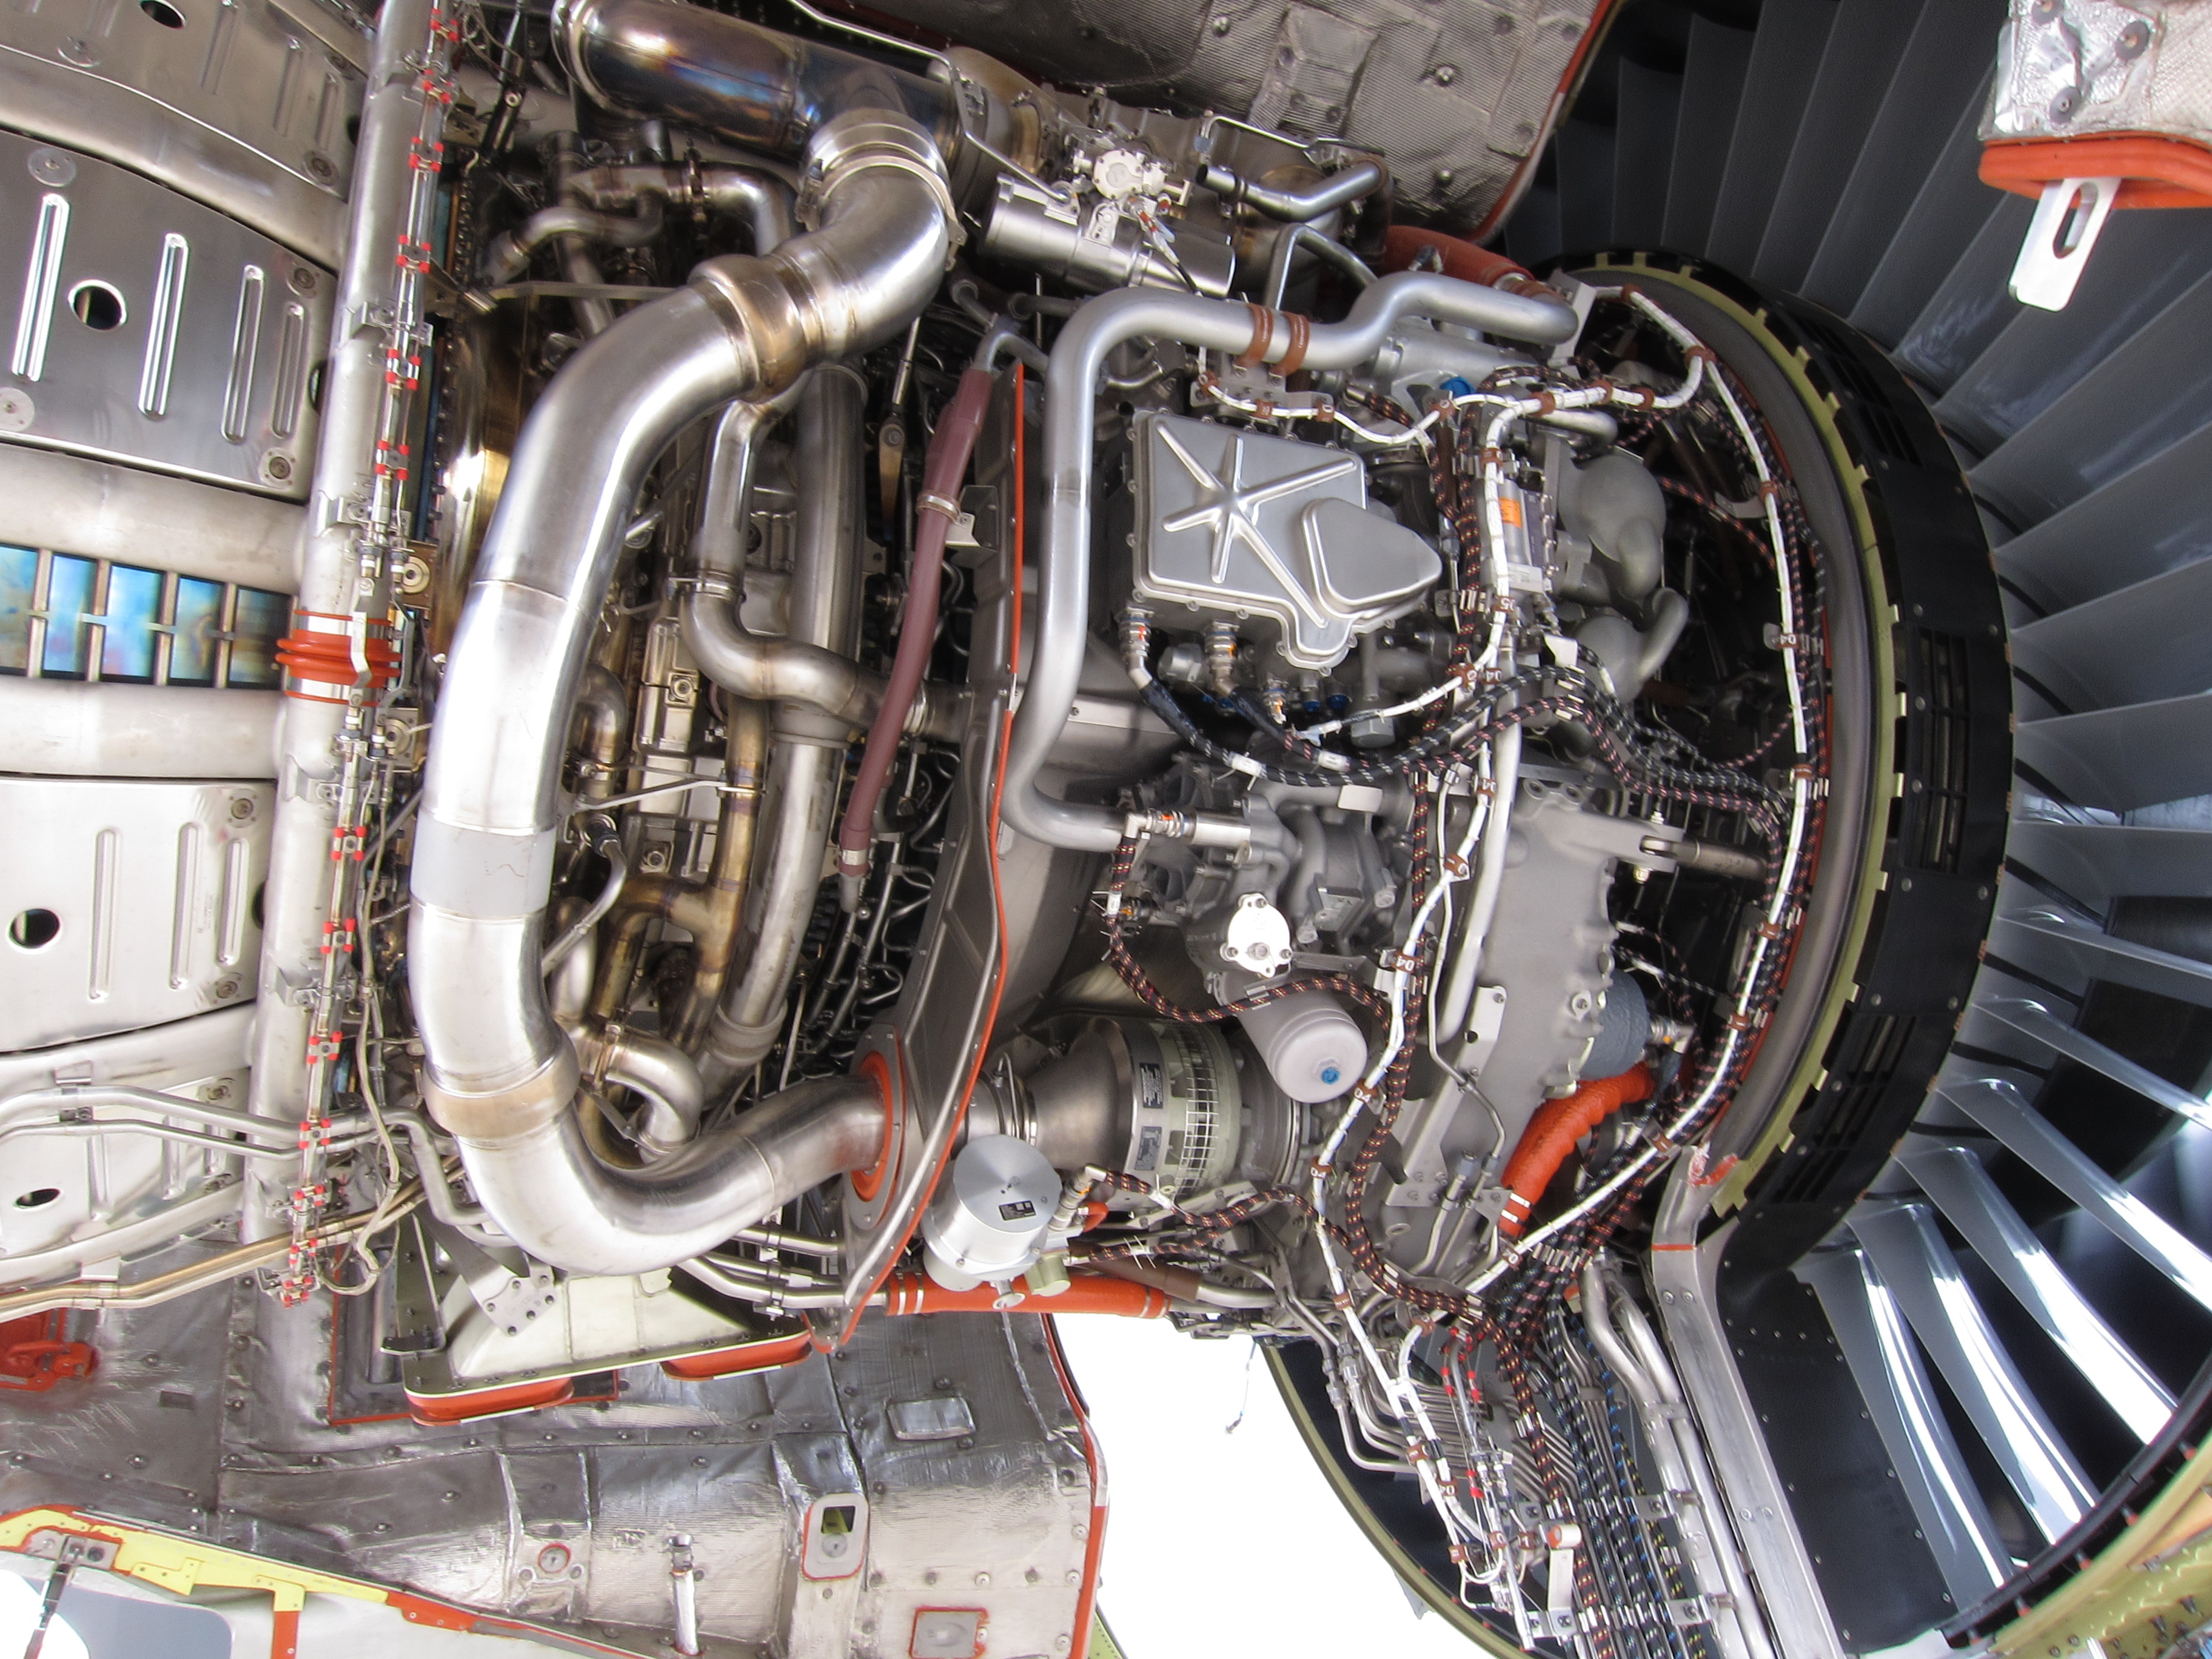
\includegraphics[height=496bp]{portada.jpg}};
 \end{scope}
}{%
 \fill[studiumLight!40!white] (0,89.5) rectangle (595.276,585.5);
 \node[text=studiumInk!45,font=\sffamily\fontsize{10}{13}\selectfont,align=center]
 at (297.638,535){Fotografía definitiva pendiente};
}
\fill[white,opacity=.91] (0,0) rectangle (595.276,89.5);
\fill[studiumInk,opacity=.96] (0,585.5) rectangle (595.276,841.89);
\node[anchor=west,text=studiumInk,font=\sffamily\bfseries\fontsize{18}{20}\selectfont,inner sep=0pt] at (51.223,38.5){STUDIUM};
\node[anchor=east,text=studiumInk,font=\sffamily\fontsize{8}{10}\selectfont,inner sep=0pt] at (544.05,38.5){EN REVISIÓN};
\fill[studiumCyan] (51.223,61.5) rectangle (80.8,63.7);
\node[anchor=west,text=studiumInk,font=\sffamily\fontsize{9}{11}\selectfont,inner sep=0pt] at (89.49,65.5){BIBLIOTECA DE INGENIERÍA};
\node[anchor=west,text=studiumCyan,font=\sffamily\bfseries\fontsize{10}{12}\selectfont,inner sep=0pt] at (51.223,608){#1};
\node[anchor=north west,text=white,text width=493pt,font=\rmfamily\bfseries\fontsize{27}{30}\selectfont,inner sep=0pt] at (51.223,627){#2};
\node[anchor=north west,text=white!82!studiumInk,text width=493pt,font=\sffamily\fontsize{11}{14}\selectfont,inner sep=0pt] at (51.223,730){#3};
\node[anchor=west,text=white,font=\sffamily\bfseries\fontsize{10}{12}\selectfont,inner sep=0pt] at (51.223,774){GRADO EN INGENIERÍA AEROESPACIAL};
\node[anchor=west,text=white!82!studiumInk,font=\sffamily\fontsize{10}{12}\selectfont,inner sep=0pt] at (51.223,789){Universidad de León};
\draw[white!75!studiumInk,line width=.4pt] (51.223,801) -- (544.05,801);
\node[anchor=west,text=white!82!studiumInk,font=\sffamily\fontsize{10}{12}\selectfont,inner sep=0pt] at (51.223,822){2026};
\node[anchor=east,text=white,font=\sffamily\bfseries\fontsize{10}{12}\selectfont,inner sep=0pt] at (544.05,822){Primera edición};
\end{scope}\end{tikzpicture}\null
\end{titlepage}\hypersetup{pageanchor=true}}

\newcommand{\creditosportada}{%
\par\noindent\begin{minipage}{\linewidth}\footnotesize
\textbf{Fotografía de portada.} Detalle del núcleo de un motor General Electric GEnx, Olivier Cleynen (21 de junio de 2011). Fuente: \href{https://commons.wikimedia.org/wiki/File:Detail_of_GEnx_turbofan_engine_core.jpg}{Wikimedia Commons}. Licencia: \href{https://creativecommons.org/licenses/by-sa/3.0/}{CC BY-SA 3.0}.
\par\noindent Se presenta con un recorte de encuadre y superposición de la composición editorial. La fotografía y su adaptación de encuadre mantienen la licencia CC BY-SA 3.0; no se atribuye al fotógrafo respaldo de esta edición.
\end{minipage}\par}

\newcommand{\caso}[2]{\begin{studiumworked}{#1}#2\end{studiumworked}}
\newcommand{\ilustra}[2]{\begin{figure}[htbp]\centering\includegraphics[width=.94\linewidth]{#1.pdf}\caption{#2}\label{fig:#1}\end{figure}}
\newcommand{\fuentes}[1]{\par\medskip\noindent{\footnotesize\textbf{Fuentes y localizadores.} #1}\par}
\newcommand{\apartado}[2]{\par\medskip\noindent\textbf{#1.} #2\par}
\newcommand{\repaso}[2]{\par\medskip\noindent\textbf{Para comprobar la comprensión.} #1\par\noindent\textit{Respuesta razonada.} #2\par}

\begin{document}\frontmatter
\portada{PROBLEMAS Y CASOS}{PROBLEMAS RESUELTOS\\Y CASOS PRÁCTICOS}{Materiales y mantenimiento de motores aeroespaciales\\35 problemas originales · 16 casos académicos}
\chapter*{Cómo utilizar este cuaderno}\addcontentsline{toc}{chapter}{Cómo utilizar este cuaderno}
Los datos y situaciones son originales y ficticios, salvo identificación expresa de una publicación oficial. Se conserva la secuencia modelo--hipótesis--desarrollo--resultado--verificación. Una comprobación numérica no valida por sí sola el modelo ni el estado de una aeronave. Las referencias de capítulo corresponden al manual de la colección.

Fecha normativa de referencia: 18 de octubre de 2026, con las versiones y pendientes indicados en el manual y los informes. Las soluciones no constituyen instrucciones aprobadas, programas aprobados ni autorizaciones de mantenimiento. En los casos puede ser correcto concluir que falta evidencia. La publicación histórica de una AD no acredita automáticamente su estado actual.
\bigskip\creditosportada
\tableofcontents\mainmatter
\chapter{Mecánica, selección y efectos térmicos}
\section{P01. Carga axial y elongación}\label{prob:P01}
\apartado{Enunciado}{Una probeta ficticia de sección uniforme recibe tracción axial centrada. Determine su respuesta elástica y explique qué propiedad faltaría para comprobar que no cede.}
\apartado{Datos}{$F=8{,}4\,\mathrm{kN}$; $A=70\,\mathrm{mm^2}$; $L_0=180\,\mathrm{mm}$; $E=72\,\mathrm{GPa}$.}
\apartado{Incógnitas}{Tensión nominal, deformación y elongación.}
\apartado{Modelo físico}{Barra uniaxial elástica lineal.}
\apartado{Hipótesis}{Pequeñas deformaciones; sección constante; sin efectos térmicos; análisis lejos de los extremos.}
\apartado{Ecuaciones}{\[\sigma=F/A,\quad\varepsilon=\sigma/E,\quad\Delta L=FL_0/(AE).\]}
\apartado{Desarrollo algebraico}{De $F=\sigma A$ se aísla $\sigma$; Hooke da $\varepsilon=\sigma/E$ y la definición de deformación da $\Delta L=\varepsilon L_0$.}
\apartado{Sustitución numérica}{$\sigma=8400/(70\times10^{-6})$ Pa; $\varepsilon=120\times10^6/(72\times10^9)$; $\Delta L=(1{,}6667\times10^{-3})(0{,}180)$ m.}
\caso{Resultado}{$\sigma=120\,\mathrm{MPa}$, $\varepsilon=1{,}6667\times10^{-3}$, $\Delta L=0{,}300\,\mathrm{mm}$.}
\apartado{Unidades}{Magnitudes de los controles numéricos: \texttt{Pa, m}. Las unidades tipográficas del resultado se muestran junto a cada valor; las conversiones se realizan antes de operar.}
\apartado{Interpretación}{La elongación responde a la rigidez axial; la tensión compara fuerza y área, sin verificar todavía cedencia.}
\apartado{Verificación}{La sustitución inversa da fuerza 8400 N y la razón elongación/longitud coincide con la deformación. La elongación es positiva para tracción.}
\apartado{Limitaciones}{Falta límite elástico y no se evalúan entallas, temperatura, fatiga ni dispersión.}
\section{P02. Dilatación impedida}\label{prob:P02}
\apartado{Enunciado}{Una barra ficticia se calienta uniformemente con sus extremos impedidos de desplazarse. Compare la dilatación libre y la tensión del modelo totalmente restringido.}
\apartado{Datos}{$L=0{,}40\,\mathrm m $; $E=110\,\mathrm{GPa}$; $\alpha=9{,}0\times10^{-6}\,\mathrm{K^{-1}}$; $\Delta T=80\,\mathrm K$.}
\apartado{Incógnitas}{Elongación libre y tensión axial con restricción total.}
\apartado{Modelo físico}{Compatibilidad térmica y elasticidad uniaxial.}
\apartado{Hipótesis}{Temperatura uniforme; apoyos rígidos; propiedades constantes; se supone régimen elástico y no se estudia pandeo.}
\apartado{Ecuaciones}{\[\varepsilon=\sigma/E+\alpha\Delta T=0,\quad\sigma=-E\alpha\Delta T,\quad\Delta L_{libre}=\alpha\Delta T L.\]}
\apartado{Desarrollo algebraico}{La compatibilidad fija $0=\sigma/E+\alpha\Delta T$, de donde $\sigma=-E\alpha\Delta T$. En expansión libre, $\Delta L=\alpha\Delta T L$.}
\apartado{Sustitución numérica}{$\Delta L=(9\times10^{-6})(80)(0{,}40)$ m; $\sigma=-(110\times10^9)(9\times10^{-6})(80)$ Pa.}
\caso{Resultado}{$\Delta L_{libre}=0{,}288\,\mathrm{mm}$; $\sigma=-79{,}2\,\mathrm{MPa}$ (compresión).}
\apartado{Unidades}{Magnitudes de los controles numéricos: \texttt{m, Pa}. Las unidades tipográficas del resultado se muestran junto a cada valor; las conversiones se realizan antes de operar.}
\apartado{Interpretación}{La compresión impide la expansión libre; una estructura flexible daría otra compatibilidad.}
\apartado{Verificación}{Al sustituir la tensión, la suma de deformación mecánica y térmica es cero. Si la temperatura no cambia, desaparecen ambas contribuciones.}
\apartado{Limitaciones}{La restricción real puede ser flexible; la plasticidad, fluencia y pandeo pueden cambiar la solución.}
\section{P03. Tensiones principales y von Mises}\label{prob:P03}
\apartado{Enunciado}{Se proporciona un estado plano uniforme en un punto. Obtenga tensiones principales y equivalente de von Mises; determine el cociente frente a un límite elástico supuesto.}
\apartado{Datos}{$\sigma_x=150$, $\sigma_y=-30$, $\tau_{xy}=40\,\mathrm{MPa}$; $\sigma_y^{mat}=300\,\mathrm{MPa}$.}
\apartado{Incógnitas}{Dos tensiones principales en el plano y equivalente.}
\apartado{Modelo físico}{Autovalores de tensor simétrico y cedencia de von Mises.}
\apartado{Hipótesis}{Tensión plana; material isótropo dúctil compatible con el criterio; pequeñas deformaciones.}
\apartado{Ecuaciones}{\[\sigma_{1,2}=60\pm\sqrt{90^2+40^2}\ \mathrm{MPa}.\]
\[\sigma_{VM}=\sqrt{150^2-150(-30)+(-30)^2+3(40)^2}\ \mathrm{MPa}.\]}
\apartado{Desarrollo algebraico}{La ecuación característica del bloque plano es $(150-s)(-30-s)-40^2=0$ en MPa. Sus raíces son $60\pm\sqrt{9700}$. Se añade la principal nula fuera del plano para el estado tridimensional.}
\apartado{Sustitución numérica}{$\sigma_{VM}=\sqrt{150^2-150(-30)+(-30)^2+3(40)^2}=\sqrt{32700}$ MPa. El cociente frente al límite es $300/\sqrt{32700}$.}
\caso{Resultado}{$\sigma_1=158{,}489$, $\sigma_2=-38{,}489\,\mathrm{MPa}$; $\sigma_{VM}=180{,}831\,\mathrm{MPa}$; cociente $1{,}659$.}
\apartado{Unidades}{Magnitudes de los controles numéricos: \texttt{MPa}. Las unidades tipográficas del resultado se muestran junto a cada valor; las conversiones se realizan antes de operar.}
\apartado{Interpretación}{El equivalente sirve para comparar cedencia en el modelo declarado, mientras las principales describen planos sin cortante.}
\apartado{Verificación}{La suma de principales del plano es 120 MPa, igual a la traza original; el determinante del bloque también se conserva.}
\apartado{Limitaciones}{El cociente no es un margen frente a grietas ni fatiga. La notación del límite material se distingue de la componente y.}
\section{P04. Pared delgada: dos direcciones de carga}\label{prob:P04}
\apartado{Enunciado}{Un cilindro cerrado idealizado recibe presión interna. Calcule tensiones de membrana y von Mises, explicando por qué no son iguales las tensiones circunferencial y longitudinal.}
\apartado{Datos}{$ p=2{,}0\,\mathrm{MPa}$; $ r=50\,\mathrm{mm}$; $ t=1{,}0\,\mathrm{mm}$.}
\apartado{Incógnitas}{Tensión circunferencial, axial y equivalente.}
\apartado{Modelo físico}{Equilibrio de membrana en cilindro de pared delgada.}
\apartado{Hipótesis}{Radio medio; presión uniforme; extremos cerrados; sin concentraciones ni flexión local; tensión radial despreciable.}
\apartado{Ecuaciones}{\[\sigma_\theta=pr/t,\quad\sigma_z=pr/(2 t),\quad\sigma_{VM}=\sqrt{\sigma_\theta^2-\sigma_\theta\sigma_z+\sigma_z^2}.\]}
\apartado{Desarrollo algebraico}{El equilibrio de un corte diametral da $2\sigma_\theta t\ell=2pr\ell$; el del extremo cerrado da $\sigma_z(2\pi rt)=p\pi r^2$. Así se obtienen las dos tensiones.}
\apartado{Sustitución numérica}{$\sigma_\theta=(2\times10^6)(0{,}05)/0{,}001$ Pa; $\sigma_z=\sigma_\theta/2$; $\sigma_{VM}=\sqrt{100^2-100(50)+50^2}$ MPa.}
\caso{Resultado}{$\sigma_\theta=100\,\mathrm{MPa}$; $\sigma_z=50\,\mathrm{MPa}$; $\sigma_{VM}=86{,}603\,\mathrm{MPa}$.}
\apartado{Unidades}{Magnitudes de los controles numéricos: \texttt{Pa, MPa}. Las unidades tipográficas del resultado se muestran junto a cada valor; las conversiones se realizan antes de operar.}
\apartado{Interpretación}{La geometría de equilibrio explica la razón dos entre tensiones; el equivalente combina ambas.}
\apartado{Verificación}{El equilibrio axial recupera la fuerza de presión sobre el extremo. Si p tiende a cero, las tensiones se anulan.}
\apartado{Limitaciones}{No se evalúan cierres, discontinuidades, ciclos, plasticidad ni un recipiente real.}
\section{P05. Energía elástica almacenada}\label{prob:P05}
\apartado{Enunciado}{Una pieza de volumen uniforme se idealiza bajo tensión uniaxial. Determine la energía elástica por volumen y la energía total.}
\apartado{Datos}{$\sigma=160\,\mathrm{MPa}$; $E=80\,\mathrm{GPa}$; $V=12\,\mathrm{cm^3}$.}
\apartado{Incógnitas}{Densidad de energía y energía.}
\apartado{Modelo físico}{Integración del trabajo en elasticidad lineal.}
\apartado{Hipótesis}{Carga uniaxial uniforme y reversible; sin energía plástica ni térmica.}
\apartado{Ecuaciones}{\[u=\int_0^{\varepsilon}E\eta\,d\eta=\sigma^2/(2 E),\quad U=u V.\]}
\apartado{Desarrollo algebraico}{Se integra $du=\sigma\,d\varepsilon=E\varepsilon\,d\varepsilon$ desde cero. Resulta $u=E\varepsilon^2/2=\sigma^2/(2E)$; $U=uV$.}
\apartado{Sustitución numérica}{$u=(160\times10^6)^2/[2(80\times10^9)]$ J/m$^3$; $U=160000(12\times10^{-6})$ J.}
\caso{Resultado}{$ u=160\,000\,\mathrm{J/m^3}$; $U=1{,}92\,\mathrm J$.}
\apartado{Unidades}{Magnitudes de los controles numéricos: \texttt{Pa, J}. Las unidades tipográficas del resultado se muestran junto a cada valor; las conversiones se realizan antes de operar.}
\apartado{Interpretación}{La energía es trabajo recuperable en el modelo elástico y no energía de rotura.}
\apartado{Verificación}{El área triangular $\sigma\varepsilon/2$ coincide con u. Las unidades de presión equivalen a energía por volumen.}
\apartado{Limitaciones}{No representa tenacidad a fractura ni energía total absorbida hasta rotura.}
\section{P06. Sensibilidad a entalla}\label{prob:P06}
\apartado{Enunciado}{Una probeta tiene un concentrador elástico y una sensibilidad a entalla especificada para el ejercicio. Compare amplificación elástica y factor efectivo de fatiga.}
\apartado{Datos}{$K_t=2{,}4$; $ q=0{,}70$; amplitud nominal $\sigma_a=60\,\mathrm{MPa}$.}
\apartado{Incógnitas}{Factor Kf y amplitudes de comparación.}
\apartado{Modelo físico}{Modelo empírico de sensibilidad a entalla.}
\apartado{Hipótesis}{El valor de q es un dato ficticio válido solo para esta situación; la curva de referencia corresponde a material sin ese detalle.}
\apartado{Ecuaciones}{\[K_f=1+q(K_t-1),\quad\sigma_{a, f}=K_f\sigma_a,\quad\sigma_{a, el}=K_t\sigma_a.\]}
\apartado{Desarrollo algebraico}{Se calcula primero $K_f=1+q(K_t-1)$. Las dos amplificaciones se aplican por separado a la misma amplitud nominal, sin multiplicar $K_f$ por $K_t$.}
\apartado{Sustitución numérica}{$K_f=1+0{,}70(2{,}4-1)=1{,}98$; $K_f\sigma_a=1{,}98(60)$ MPa; $K_t\sigma_a=2{,}4(60)$ MPa.}
\caso{Resultado}{$K_f=1{,}98$; $\sigma_{a,f}=118{,}8\,\mathrm{MPa}$; pico elástico de amplitud $144\,\mathrm{MPa}$.}
\apartado{Unidades}{Magnitudes de los controles numéricos: \texttt{adimensional, MPa}. Las unidades tipográficas del resultado se muestran junto a cada valor; las conversiones se realizan antes de operar.}
\apartado{Interpretación}{El efecto de entalla en fatiga es menor que la concentración elástica para la sensibilidad adoptada.}
\apartado{Verificación}{Con q=0 resulta Kf=1 y con q=1 resulta Kf=Kt; ambos límites se satisfacen.}
\apartado{Limitaciones}{Kf no predice el campo local de plasticidad ni debe aplicarse de nuevo si la curva ya corresponde a la pieza entallada.}
\section{P34. Masa con restricción resistente}\label{prob:P34}
\apartado{Enunciado}{Compare masas ideales de dos barras que deben transmitir la misma fuerza. La geometría se adapta al mismo criterio resistente ficticio.}
\apartado{Datos}{$F=40\,\mathrm{kN}$; $L=0{,}50\,\mathrm m $; A:$\rho=2800\,\mathrm{kg/m^3}$,$\sigma_{adm}=300\,\mathrm{MPa}$; B:4500 kg/m\(^{3}\) y 650 MPa.}
\apartado{Incógnitas}{Secciones y masas mínimas del modelo.}
\apartado{Modelo físico}{Barra traccionada limitada por tensión admisible.}
\apartado{Hipótesis}{Longitud y carga iguales; se puede elegir libremente área; no hay restricción de rigidez, unión ni temperatura.}
\apartado{Ecuaciones}{\[A_{min}=F/\sigma_{adm},\quad m_{min}=\rho FL/\sigma_{adm}.\]}
\apartado{Desarrollo algebraico}{El área mínima es $F/\sigma_{adm}$. Sustituir en $m=\rho AL$ da $m=\rho FL/\sigma_{adm}$, con un área distinta para cada material.}
\apartado{Sustitución numérica}{$m_A=2800(40000)(0{,}50)/(300\times10^6)$ kg; $m_B=4500(40000)(0{,}50)/(650\times10^6)$ kg.}
\caso{Resultado}{$A_A=133{,}333\,\mathrm{mm^2}$, $A_B=61{,}538\,\mathrm{mm^2}$; $ m_A=0.18667\,\mathrm{kg}$, $ m_B=0.13846\,\mathrm{kg}$.}
\apartado{Unidades}{Magnitudes de los controles numéricos: \texttt{kg}. Las unidades tipográficas del resultado se muestran junto a cada valor; las conversiones se realizan antes de operar.}
\apartado{Interpretación}{El material más denso puede producir menor masa cuando gobierna resistencia y cambia el área.}
\apartado{Verificación}{Las tensiones de cada sección recuperan el admisible. El material más denso produce menor masa en este problema.}
\apartado{Limitaciones}{La conclusión cambia si gobierna rigidez, estabilidad, fabricación o daño.}

\chapter{Fractura y tolerancia al daño}
\section{P07. Intensidad aplicada a una grieta de borde}\label{prob:P07}
\apartado{Enunciado}{Se idealiza una grieta de borde bajo tracción. Compare la intensidad con una tenacidad supuesta aplicable y explique el alcance de la comparación.}
\apartado{Datos}{$ a=1{,}8\,\mathrm{mm}$ (longitud desde el borde); $Y=1{,}12$ constante; $\sigma=210\,\mathrm{MPa}$; $K_{IC}=42\,\mathrm{MPa\sqrt m}$.}
\apartado{Incógnitas}{KI y cociente KI/KIC.}
\apartado{Modelo físico}{MFEL de modo I con factor geométrico dado.}
\apartado{Hipótesis}{Pequeña plastificación y tenacidad de deformación plana asumidas; carga remota; no crecimiento subcrítico.}
\apartado{Ecuaciones}{\[K_I=Y\sigma\sqrt{\pi a}.\]}
\apartado{Desarrollo algebraico}{Con $Y$ dado, se evalúa $K_I$ y se divide por la tenacidad supuesta: $K_I/K_{IC}=Y\sigma\sqrt{\pi a}/K_{IC}$. No se sustituye $a$ por una longitud total.}
\apartado{Sustitución numérica}{$K_I=1{,}12(210)\sqrt{\pi(0{,}0018)}$ MPa$\sqrt{\mathrm m}$; el cociente divide ese valor por 42 en la misma unidad.}
\caso{Resultado}{$K_I=17.6868\,\mathrm{MPa\sqrt m}$; $K_I/K_{IC}=0.4211$.}
\apartado{Unidades}{Magnitudes de los controles numéricos: \texttt{MPa*m\textasciicircum{}0.5}. Las unidades tipográficas del resultado se muestran junto a cada valor; las conversiones se realizan antes de operar.}
\apartado{Interpretación}{La intensidad resulta inferior a la tenacidad supuesta, con una conclusión estática y condicionada.}
\apartado{Verificación}{Elevar al cuadrado permite comprobar $K_I^2/(Y^2\sigma^2)=\pi a $. La comparación resulta inferior a uno dentro del modelo.}
\apartado{Limitaciones}{No se han comprobado espesor ni fatiga o corrosión; no es criterio de aceptación en servicio.}
\section{P08. Tamaño crítico y longitud total}\label{prob:P08}
\apartado{Enunciado}{Una placa muy ancha contiene una grieta central pasante. Calcule el tamaño crítico y la tensión crítica para un defecto inicial, conservando la definición de semilongitud.}
\apartado{Datos}{$K_{IC}=36\,\mathrm{MPa\sqrt m}$; $\sigma=240\,\mathrm{MPa}$; $Y=1$; longitud total inicial $2a_i=3\,\mathrm{mm}$.}
\apartado{Incógnitas}{$a_c$, $2a_c$ y tensión crítica para $a_i$.}
\apartado{Modelo físico}{Criterio estático KI=KIC en MFEL.}
\apartado{Hipótesis}{Y constante; tenacidad aplicable; carga uniforme y pequeña zona plástica.}
\apartado{Ecuaciones}{\[a_c=(K_{IC}/\sigma)^2/\pi,\quad \sigma_c=K_{IC}/\sqrt{\pi a_i}.\]}
\apartado{Desarrollo algebraico}{Elevar $K_{IC}=\sigma\sqrt{\pi a_c}$ al cuadrado y aislar da $a_c=K_{IC}^2/(\pi\sigma^2)$. Para el defecto inicial se aísla tensión, no tamaño.}
\apartado{Sustitución numérica}{$a_i=0{,}0015$ m; $a_c=(36/240)^2/\pi$ m; $\sigma_c=36/\sqrt{\pi(0{,}0015)}$ MPa.}
\caso{Resultado}{$ a_c=7.1620\,\mathrm{mm}$; $2a_c=14.3239\,\mathrm{mm}$; $\sigma_c=524.423\,\mathrm{MPa}$.}
\apartado{Unidades}{Magnitudes de los controles numéricos: \texttt{m, MPa}. Las unidades tipográficas del resultado se muestran junto a cada valor; las conversiones se realizan antes de operar.}
\apartado{Interpretación}{La longitud crítica total duplica la semilongitud; el defecto inicial requiere su propia tensión crítica.}
\apartado{Verificación}{Sustituir $a_c$ en $K_I$ recupera $36\,\mathrm{MPa\sqrt m}$. Duplicar tensión reduce el tamaño crítico a un cuarto si $Y$ permanece constante.}
\apartado{Limitaciones}{Falta comprobar cedencia, ligamento y espesor; no hay crecimiento por fatiga en esta solución.}
\section{P09. Cribado de deformación plana}\label{prob:P09}
\apartado{Enunciado}{Se dispone de un valor candidato de tenacidad y una chapa. Calcule la dimensión de cribado y compruebe si el espesor la satisface.}
\apartado{Datos}{$K=48\,\mathrm{MPa\sqrt m}$; $\sigma_y=900\,\mathrm{MPa}$; $B=5\,\mathrm{mm}$.}
\apartado{Incógnitas}{Dimensión $2{,}5(K/\sigma_y)^2$ y comparación con espesor.}
\apartado{Modelo físico}{Condición dimensional de cribado de validez de tenacidad plana.}
\apartado{Hipótesis}{Se utiliza como condición necesaria de estudio; no como certificación de ensayo normalizado.}
\apartado{Ecuaciones}{\[\ell_{min}=2{,}5(K/\sigma_y)^2.\]}
\apartado{Desarrollo algebraico}{Se evalúa la longitud de cribado y después se compara con el espesor: $B/\ell_{min}$. No se invierte el sentido de la desigualdad.}
\apartado{Sustitución numérica}{$\ell_{min}=2{,}5(48/900)^2$ m $=7{,}111$ mm; $B/\ell_{min}=5/7{,}111<1$.}
\caso{Resultado}{$\ell_{min}=7{,}111\,\mathrm{mm}>B=5\,\mathrm{mm}$; el espesor no satisface el cribado.}
\apartado{Unidades}{Magnitudes de los controles numéricos: \texttt{m}. Las unidades tipográficas del resultado se muestran junto a cada valor; las conversiones se realizan antes de operar.}
\apartado{Interpretación}{El espesor es insuficiente para el cribado, por lo que la denominación de tenacidad plana no está demostrada.}
\apartado{Verificación}{El cociente tiene unidades de raíz de longitud; su cuadrado es longitud.}
\apartado{Limitaciones}{Faltan condiciones de probeta, ligamento, carga y norma. No se debe denominar KIC válido al valor candidato solo por disponer de él.}
\section{P10. Factor geométrico variable}\label{prob:P10}
\apartado{Enunciado}{Una solución idealizada de placa de anchura total W utiliza el factor especificado. Obtenga la semilongitud crítica por resolución implícita y compárela con Y=1.}
\apartado{Datos}{$W=80\,\mathrm{mm}$; $\sigma=180\,\mathrm{MPa}$; $K_{IC}=30\,\mathrm{MPa\sqrt m}$; $Y=\sqrt{\sec(\pi a/W)}$; $0<a<W/2$.}
\apartado{Incógnitas}{Raíz ac y comparación de anchura infinita.}
\apartado{Modelo físico}{MFEL con solución geométrica expresamente dada.}
\apartado{Hipótesis}{Placa central pasante; convención W de anchura total; dominio de Y indicado; pequeña plastificación supuesta.}
\apartado{Ecuaciones}{\[180\sqrt{\pi a/\cos(\pi a/0{,}08)}=30.\]}
\apartado{Desarrollo algebraico}{La ecuación implícita es $f(a)=180\sqrt{\pi a/\cos(\pi a/0{,}08)}-30=0$. Se usa bisección en $0<a<0{,}04$ m; el argumento es positivo y la función crece en el dominio.}
\apartado{Sustitución numérica}{La raíz se sustituye en $180\sqrt{\pi a/\cos(\pi a/0{,}08)}$. El valor de intensidad debe recuperar 30. La comparación de placa infinita es $a_{\infty}=(30/180)^2/\pi$ m.}
\caso{Resultado}{$ a_c=8.36874\,\mathrm{mm}$; con $Y=1$, $ a_{c,\infty}=8.84194\,\mathrm{mm}$.}
\apartado{Unidades}{Magnitudes de los controles numéricos: \texttt{MPa*m\textasciicircum{}0.5}. Las unidades tipográficas del resultado se muestran junto a cada valor; las conversiones se realizan antes de operar.}
\apartado{Interpretación}{La corrección por anchura eleva intensidad y reduce el tamaño crítico respecto a la placa infinita.}
\apartado{Verificación}{La sustitución de la raíz en la expresión completa recupera 30 MPa raíz de m; el tamaño finito es menor porque Y>1. Se comprueba ac<W/2.}
\apartado{Limitaciones}{No se extrapola esta solución a una grieta de borde, superficie, otro sistema de carga o plasticidad extensa.}

\chapter{Fatiga y propagación}
\section{P11. Carga repetida y Goodman}\label{prob:P11}
\apartado{Enunciado}{Una probeta se carga desde cero hasta un máximo positivo. Use el criterio de Goodman dado para hallar el máximo nominal compatible con el límite de la aproximación.}
\apartado{Datos}{$S_e=240\,\mathrm{MPa}$; $S_u=800\,\mathrm{MPa}$; $R=0$; sin factor de entalla.}
\apartado{Incógnitas}{Tensión máxima y amplitud.}
\apartado{Modelo físico}{Goodman lineal con tensión media de tracción.}
\apartado{Hipótesis}{Datos ficticios para condiciones compatibles; no plasticidad y no factor de seguridad adicional.}
\apartado{Ecuaciones}{\[\sigma_a=\sigma_m=\sigma_{max}/2,\quad\sigma_{max}=2/(1/S_e+1/S_u).\]}
\apartado{Desarrollo algebraico}{Para $R=0$, $\sigma_a=\sigma_m=\sigma_{max}/2$. Goodman se convierte en $(\sigma_{max}/2)(1/S_e+1/S_u)=1$.}
\apartado{Sustitución numérica}{$\sigma_{max}=2/(1/240+1/800)$ MPa. Amplitud y media son la mitad de ese máximo.}
\caso{Resultado}{$\sigma_{max}=369{,}231\,\mathrm{MPa}$; $\sigma_a=\sigma_m=184{,}615\,\mathrm{MPa}$.}
\apartado{Unidades}{Magnitudes de los controles numéricos: \texttt{MPa}. Las unidades tipográficas del resultado se muestran junto a cada valor; las conversiones se realizan antes de operar.}
\apartado{Interpretación}{La tensión media consume parte del margen del modelo de Goodman; máximo y amplitud deben distinguirse.}
\apartado{Verificación}{La suma de los dos cocientes de Goodman es 1. Con media nula el criterio recuperaría amplitud Se.}
\apartado{Limitaciones}{No representa vida infinita en corrosión ni una curva específica de pieza; Goodman es aproximación.}
\section{P12. Ajuste de una ley S--N}\label{prob:P12}
\apartado{Enunciado}{Dos puntos ficticios de una curva completamente alternante se ajustan por una recta en logaritmos. Obtenga coeficientes y vida interpolada a otra amplitud.}
\apartado{Datos}{$(N_1,\sigma_{a1})=(10^4,400\,\mathrm{MPa})$; $(N_2,\sigma_{a2})=(10^6,220\,\mathrm{MPa})$; amplitud objetivo 280 MPa.}
\apartado{Incógnitas}{A, b y ciclos.}
\apartado{Modelo físico}{Basquin con $\sigma_a=AN^b$, usando ciclos y no reversiones.}
\apartado{Hipótesis}{R=-1; misma superficie y temperatura; se interpola dentro del dominio de los dos datos.}
\apartado{Ecuaciones}{\[b=\ln(\sigma_{a 2}/\sigma_{a 1})/\ln(N_2/N_1),\quad A=\sigma_{a 1}/N_1^b,\quad N=(280/A)^{1/b}.\]}
\apartado{Desarrollo algebraico}{Al dividir las dos leyes $\sigma_a=AN^b$ se elimina $A$: $\sigma_{a2}/\sigma_{a1}=(N_2/N_1)^b$. Un logaritmo permite aislar $b$, y después $A=\sigma_{a1}/N_1^b$.}
\apartado{Sustitución numérica}{$b=\ln(220/400)/\ln(10^6/10^4)$; $A=400/(10^4)^b$ MPa; $N=(280/A)^{1/b}$ ciclos.}
\caso{Resultado}{$ b=-0.129819$; $A=1322.3140\,\mathrm{MPa}$; $N=156033.6$ ciclos.}
\apartado{Unidades}{Magnitudes de los controles numéricos: \texttt{adimensional}. Las unidades tipográficas del resultado se muestran junto a cada valor; las conversiones se realizan antes de operar.}
\apartado{Interpretación}{La interpolación asigna una vida solo dentro del tramo y convención de la curva ajustada.}
\apartado{Verificación}{Sustituir $10^4$ y $10^6$ ciclos recupera 400 y 220 MPa. La vida objetivo queda entre ambas.}
\apartado{Limitaciones}{Dos puntos no describen dispersión ni justifican extrapolar; no se aplica con otra razón R sin corrección.}
\section{P13. Miner con un nivel restante}\label{prob:P13}
\apartado{Enunciado}{Un bloque contiene una contribución conocida y otra desconocida. Determine cuántos ciclos del segundo nivel completan el daño lineal unitario.}
\apartado{Datos}{$ n_1=18\,000$, $N_1=120\,000$; $N_2=30\,000$; criterio $D=1$.}
\apartado{Incógnitas}{Número de ciclos $n_2$.}
\apartado{Modelo físico}{Acumulación lineal de Miner.}
\apartado{Hipótesis}{Niveles de carga definidos por vidas de referencia compatibles; no interacción ni efecto de secuencia.}
\apartado{Ecuaciones}{\[n_1/N_1+n_2/N_2=1,\quad n_2=N_2(1-n_1/N_1).\]}
\apartado{Desarrollo algebraico}{De $n_1/N_1+n_2/N_2=1$ se obtiene $n_2=N_2(1-n_1/N_1)$. El paréntesis debe ser no negativo para que exista margen en este modelo.}
\apartado{Sustitución numérica}{$n_2=30000(1-18000/120000)=30000(0{,}85)$ ciclos.}
\caso{Resultado}{$ n_2=25\,500$ ciclos.}
\apartado{Unidades}{Magnitudes de los controles numéricos: \texttt{adimensional}. Las unidades tipográficas del resultado se muestran junto a cada valor; las conversiones se realizan antes de operar.}
\apartado{Interpretación}{El daño previo consume una fracción de la vida idealizada; la vida restante depende del siguiente nivel.}
\apartado{Verificación}{La suma $0{,}15+25500/30000$ es uno y $n_2<N_2$.}
\apartado{Limitaciones}{La igualdad D=1 no es una fecha determinista de fallo real y no representa el orden de los niveles.}
\section{P14. Bloques y acumulación}\label{prob:P14}
\apartado{Enunciado}{Una misión ficticia repite dos niveles. Calcule daño por misión y número de misiones completas antes del criterio lineal.}
\apartado{Datos}{$ n_1=120$, $N_1=60\,000$; $ n_2=30$, $N_2=10\,000$.}
\apartado{Incógnitas}{Daño y misiones.}
\apartado{Modelo físico}{Miner con bloques idénticos.}
\apartado{Hipótesis}{Datos del mismo modelo de vida; secuencia no representada; sin dispersión.}
\apartado{Ecuaciones}{\[D_b=120/60000+30/10000,\quad B=1/D_b.\]}
\apartado{Desarrollo algebraico}{El daño de un bloque es suma de sus fracciones. Tras $B$ bloques, $D=B D_b$; el criterio unitario da $B=1/D_b$.}
\apartado{Sustitución numérica}{$D_b=120/60000+30/10000=0{,}005$; $B=1/0{,}005=200$ bloques.}
\caso{Resultado}{$D_b=0{,}005$; $B=200$ misiones al criterio. Tras 199, $D=0{,}995$.}
\apartado{Unidades}{Magnitudes de los controles numéricos: \texttt{adimensional}. Las unidades tipográficas del resultado se muestran junto a cada valor; las conversiones se realizan antes de operar.}
\apartado{Interpretación}{Los bloques acumulan daño linealmente y el fallo idealizado puede caer dentro de un bloque.}
\apartado{Verificación}{Multiplicar 200 por 0,005 recupera 1. La suma de fracciones es adimensional.}
\apartado{Limitaciones}{El umbral académico no implica autorización para volar 199 misiones; faltan márgenes y validación física.}
\section{P15. K máximo y rango de intensidad}\label{prob:P15}
\apartado{Enunciado}{Se idealiza una grieta sometida a carga cíclica de tracción. Calcule las intensidades y distinga las comprobaciones de crecimiento e inestabilidad.}
\apartado{Datos}{$ a=2{,}5\,\mathrm{mm}$; $Y=1{,}1$; $\sigma_{max}=200$ y $\sigma_{min}=40\,\mathrm{MPa}$; $K_{IC}=35\,\mathrm{MPa\sqrt m}$.}
\apartado{Incógnitas}{$K_{max}$, $K_{min}$, $\Delta K$ y $R$.}
\apartado{Modelo físico}{MFEL lineal sin cierre de grieta.}
\apartado{Hipótesis}{Ambos extremos de carga en tracción; Y y a constantes durante el ciclo; tenacidad supuesta aplicable.}
\apartado{Ecuaciones}{\[K_{max, min}=Y\sigma_{max, min}\sqrt{\pi a},\quad\Delta K=Y(\sigma_{max}-\sigma_{min})\sqrt{\pi a}.\]}
\apartado{Desarrollo algebraico}{Se calcula $\sigma_{min}=R\sigma_{max}$ y después $\Delta\sigma=(1-R)\sigma_{max}$. La misma geometría permite escribir $\Delta K=(1-R)K_{max}$.}
\apartado{Sustitución numérica}{$R=40/200=0{,}2$; $\Delta\sigma=200-40=160$ MPa. $K_{max}=1{,}1(200)\sqrt{\pi(0{,}0025)}$ y $\Delta K=1{,}1(160)\sqrt{\pi(0{,}0025)}$, ambos en MPa$\sqrt{\mathrm m}$.}
\caso{Resultado}{$K_{max}=19.4970$; $K_{min}=3.8994$; $\Delta K=15.5976\,\mathrm{MPa\sqrt m}$; $R=0{,}20$.}
\apartado{Unidades}{Magnitudes de los controles numéricos: \texttt{MPa*m\textasciicircum{}0.5}. Las unidades tipográficas del resultado se muestran junto a cada valor; las conversiones se realizan antes de operar.}
\apartado{Interpretación}{La intensidad máxima y el rango responden a preguntas físicas distintas: inestabilidad y crecimiento.}
\apartado{Verificación}{$K_{min}/K_{max}=R$ y $K_{max}-K_{min}=\Delta K$. La intensidad máxima queda por debajo de la tenacidad supuesta en el modelo.}
\apartado{Limitaciones}{Un $\Delta K$ positivo no garantiza validez de Paris: se necesita dominio de crecimiento, umbral, razón de carga y condiciones. La comparación estática no excluye propagación.}
\section{P16. Vida de propagación: Paris m=3}\label{prob:P16}
\apartado{Enunciado}{Una grieta central idealizada crece en la región de Paris. Calcule ciclos entre dos semilongitudes. El objetivo es vida de propagación, no vida total desde material sin defecto.}
\apartado{Datos}{$ a_i=1{,}0\,\mathrm{mm}$; $ a_f=6{,}0\,\mathrm{mm}$; $Y=1$; $\Delta\sigma=110\,\mathrm{MPa}$; $ m=3$; $C=2\times10^{-12}\,\mathrm{m/ciclo}/(\mathrm{MPa\sqrt m})^3$.}
\apartado{Incógnitas}{Ciclos N.}
\apartado{Modelo físico}{Paris con rango constante y Yconstante.}
\apartado{Hipótesis}{Grieta larga; región intermedia válida durante todo el intervalo supuesto; sin cierre, retardos ni iniciación. El estado final se supone admisible por un criterio independiente.}
\apartado{Ecuaciones}{\[N=\frac{2(a_i^{-1/2}-a_f^{-1/2})}{C(\Delta\sigma\sqrt\pi)^3}.\]}
\apartado{Desarrollo algebraico}{La separación da $dN=a^{-3/2}da/[C(\Delta\sigma\sqrt\pi)^3]$. La primitiva es $-2a^{-1/2}$ y al evaluar extremos queda una vida positiva.}
\apartado{Sustitución numérica}{$N=2(0{,}001^{-1/2}-0{,}006^{-1/2})/[2\times10^{-12}(110\sqrt\pi)^3]$ ciclos.}
\caso{Resultado}{$N=2524856.2$ ciclos de propagación.}
\apartado{Unidades}{Magnitudes de los controles numéricos: \texttt{adimensional}. Las unidades tipográficas del resultado se muestran junto a cada valor; las conversiones se realizan antes de operar.}
\apartado{Interpretación}{La vida calculada cubre crecimiento entre tamaños, sin añadir iniciación ni certificar detectabilidad.}
\apartado{Verificación}{La derivada de la primitiva reproduce $a^{-3/2}$; una cuadratura numérica independiente se registra en el informe. N crece al reducir el rango de tensión.}
\apartado{Limitaciones}{No se ha comprobado Kmax contra tenacidad ni POD de la inspección; no es intervalo autorizado.}
\section{P17. Paris m=2: el caso logarítmico}\label{prob:P17}
\apartado{Enunciado}{Calcule vida entre dos tamaños para una ley de Paris con exponente 2 y explique por qué no se usa la expresión de potencia con denominador 1-m/2.}
\apartado{Datos}{$ a_i=0{,}8\,\mathrm{mm}$; $ a_f=5\,\mathrm{mm}$; $Y=1$; $\Delta\sigma=90\,\mathrm{MPa}$; $ m=2$; $C=5\times10^{-10}\,\mathrm{m/ciclo}/(\mathrm{MPa\sqrt m})^2$.}
\apartado{Incógnitas}{N.}
\apartado{Modelo físico}{Integración de da/[C(Delta K)\textasciicircum{}2].}
\apartado{Hipótesis}{Región de Paris y condiciones constantes asumidas; mismos límites físicos que P16.}
\apartado{Ecuaciones}{\[N=\frac{\ln(a_f/a_i)}{C(\Delta\sigma\sqrt\pi)^2}.\]}
\apartado{Desarrollo algebraico}{Con exponente dos, el integrando es proporcional a $1/a$. Se integra como $\ln a$; el cociente de tamaños dentro del logaritmo es adimensional.}
\apartado{Sustitución numérica}{$N=\ln(0{,}005/0{,}0008)/[5\times10^{-10}(90\sqrt\pi)^2]$ ciclos.}
\caso{Resultado}{$N=144031.8$ ciclos.}
\apartado{Unidades}{Magnitudes de los controles numéricos: \texttt{adimensional}. Las unidades tipográficas del resultado se muestran junto a cada valor; las conversiones se realizan antes de operar.}
\apartado{Interpretación}{El exponente dos cambia la primitiva a un logaritmo y requiere mantener unidades del coeficiente.}
\apartado{Verificación}{La cuadratura del integrando coincide con el logaritmo. Si los tamaños final e inicial coinciden, el logaritmo y la vida de propagación son cero.}
\apartado{Limitaciones}{Los coeficientes no se reutilizan para otro exponente o sistema de unidades.}
\section{P18. Un intervalo de inspección académico}\label{prob:P18}
\apartado{Enunciado}{Una grieta detectable idealizada crece hasta un tamaño final previamente fijado. Estime vida de propagación y un intervalo académico del 40\% de esa vida.}
\apartado{Datos}{$ a_i=0{,}7\,\mathrm{mm}$; $ a_f=4\,\mathrm{mm}$; $Y=1$; $\Delta\sigma=100\,\mathrm{MPa}$; $C=1{,}5\times10^{-12}\,\mathrm{m/ciclo}/(\mathrm{MPa\sqrt m})^3$; $ m=3$.}
\apartado{Incógnitas}{Vida de propagación e intervalo académico.}
\apartado{Modelo físico}{Paris y fracción de vida expresamente impuesta por el ejercicio.}
\apartado{Hipótesis}{Región de Paris supuesta; tamaño inicial no representa una POD validada; el factor 0,4 no es reglamentario.}
\apartado{Ecuaciones}{\[N=2(a_i^{-1/2}-a_f^{-1/2})/[C(\Delta\sigma\sqrt\pi)^3],\quad I=0{,}4 N.\]}
\apartado{Desarrollo algebraico}{Se integra Paris con exponente tres antes de aplicar la fracción: $I=0{,}4N$. Si se exige entero, se redondea el intervalo hacia abajo.}
\apartado{Sustitución numérica}{$N=2(0{,}0007^{-1/2}-0{,}004^{-1/2})/[1{,}5\times10^{-12}(100\sqrt\pi)^3]$ ciclos; después se multiplica por $0{,}4$.}
\caso{Resultado}{$N=5264311.3$ ciclos; $I=2105724.5$ ciclos, o 2105724 ciclos enteros redondeados hacia abajo.}
\apartado{Unidades}{Magnitudes de los controles numéricos: \texttt{adimensional}. Las unidades tipográficas del resultado se muestran junto a cada valor; las conversiones se realizan antes de operar.}
\apartado{Interpretación}{La fracción académica reduce el intervalo respecto a la vida de propagación, sin ser regla reglamentaria.}
\apartado{Verificación}{La fracción del intervalo respecto a la vida calculada es 0,4. Una integración numérica independiente contrasta la vida.}
\apartado{Limitaciones}{No se define un intervalo real sin espectro, tenacidad, probabilidad de detección, dispersión y aprobación aplicable.}

\chapter{Fluencia y exposición térmica}
\section{P19. Sensibilidad a tensión de fluencia}\label{prob:P19}
\apartado{Enunciado}{A temperatura constante, una ley normalizada de Norton predice la tasa secundaria. Obtenga la tasa y la deformación acumulada durante una permanencia.}
\apartado{Datos}{$\dot\varepsilon_1=2\times10^{-8}\,\mathrm{s^{-1}}$ a $\sigma_1=200\,\mathrm{MPa}$; $ n=5$; $\sigma_2=240\,\mathrm{MPa}$; permanencia 20 h.}
\apartado{Incógnitas}{Tasa 2 e incremento de deformación.}
\apartado{Modelo físico}{Norton a temperatura fija en un mecanismo dado.}
\apartado{Hipótesis}{Misma microestructura y régimen; solo tramo secundario; tensión constante durante 20 h.}
\apartado{Ecuaciones}{\[\dot\varepsilon_2=\dot\varepsilon_1(\sigma_2/\sigma_1)^n,\quad\Delta\varepsilon=\dot\varepsilon_2 t.\]}
\apartado{Desarrollo algebraico}{A temperatura fija se divide la ley de Norton en ambos estados y se elimina el prefactor: $\dot\varepsilon_2/\dot\varepsilon_1=(\sigma_2/\sigma_1)^n$.}
\apartado{Sustitución numérica}{$\dot\varepsilon_2=2\times10^{-8}(240/200)^5$ s$^{-1}$; $\Delta\varepsilon=\dot\varepsilon_2(20\times3600)$.}
\caso{Resultado}{$\dot\varepsilon_2=4{,}97664\times10^{-8}\,\mathrm{s^{-1}}$; $\Delta\varepsilon=0{,}00358318$ (0,3583\%).}
\apartado{Unidades}{Magnitudes de los controles numéricos: \texttt{1/s, adimensional}. Las unidades tipográficas del resultado se muestran junto a cada valor; las conversiones se realizan antes de operar.}
\apartado{Interpretación}{La potencia de tensión amplifica un cambio moderado de carga; el tiempo convierte tasa en deformación.}
\apartado{Verificación}{La razón es adimensional; tasa por tiempo da deformación. Al igualar tensiones se recupera la tasa inicial.}
\apartado{Limitaciones}{No incluye fluencia primaria/terciaria, temperatura variable ni tiempo a rotura.}
\section{P20. Sensibilidad conjunta a tensión y temperatura}\label{prob:P20}
\apartado{Enunciado}{Una ley de Norton--Arrhenius se expresa por cociente respecto a un estado de referencia. Calcule la tasa al cambiar tensión y temperatura.}
\apartado{Datos}{$\dot\varepsilon_1=10^{-8}\,\mathrm{s^{-1}}$; $T_1=930\,\mathrm K$, $T_2=980\,\mathrm K$; $\sigma_1=180$, $\sigma_2=200\,\mathrm{MPa}$; $ n=4$; $Q=220\,\mathrm{kJ/mol}$.}
\apartado{Incógnitas}{Razón de tasas y tasa 2.}
\apartado{Modelo físico}{Activación térmica con un único mecanismo.}
\apartado{Hipótesis}{Mismos Q y n y estado; constantes con unidades coherentes; temperatura absoluta.}
\apartado{Ecuaciones}{\[\dot\varepsilon_2/\dot\varepsilon_1=(200/180)^4\exp[-220000/R(1/980-1/930)].\]}
\apartado{Desarrollo algebraico}{Al dividir Norton--Arrhenius se eliminan constantes comunes y se conservan razón de tensión y diferencia de inversas de temperatura. Cada factor es adimensional.}
\apartado{Sustitución numérica}{$r=(200/180)^4\exp[-220000(1/980-1/930)/8{,}314462618]$; $\dot\varepsilon_2=r\,10^{-8}$ s$^{-1}$.}
\caso{Resultado}{Factor térmico 4.26998; razón total 6.50812; $\dot\varepsilon_2=6.508119\times10^{-8}\,\mathrm{s^{-1}}$.}
\apartado{Unidades}{Magnitudes de los controles numéricos: \texttt{adimensional}. Las unidades tipográficas del resultado se muestran junto a cada valor; las conversiones se realizan antes de operar.}
\apartado{Interpretación}{Ambos cambios elevan la tasa del mecanismo asumido; no se deduce por ello una vida de rotura.}
\apartado{Verificación}{La tasa aumenta por ambos cambios. El exponente es adimensional y la temperatura no se introduce en grados Celsius.}
\apartado{Limitaciones}{No se extrapola a una transición de mecanismo ni se deduce tiempo a rotura de una tasa aislada.}
\section{P21. Larson--Miller a tensión fija}\label{prob:P21}
\apartado{Enunciado}{Una correlación ficticia de rotura se considera válida en dos temperaturas a igual tensión. Estime el tiempo equivalente y compruebe el parámetro.}
\apartado{Datos}{$T_1=900\,\mathrm K$; $ t_1=10000\,\mathrm h $; $T_2=950\,\mathrm K$; $C_{LM}=20$, calibrado con horas.}
\apartado{Incógnitas}{Tiempo $t_2$ y parámetro $P$.}
\apartado{Modelo físico}{Igualdad del parámetro Larson--Miller a tensión fija.}
\apartado{Hipótesis}{Mismo material, estado, mecanismo y tensión; correlación supuesta válida.}
\apartado{Ecuaciones}{\[P=T_1(C_{LM}+\log_{10}t_1),\quad \log_{10}t_2=P/T_2-C_{LM}.\]}
\apartado{Desarrollo algebraico}{La igualdad de parámetros a igual tensión permite aislar $\log_{10}t_2=P/T_2-C_{LM}$; aplicar la potencia de diez devuelve horas.}
\apartado{Sustitución numérica}{$P=900(20+\log_{10}10000)=21600$ K; $t_2=10^{21600/950-20}$ h.}
\caso{Resultado}{$ t_2=545.5595\,\mathrm h $; $P=21600\,\mathrm K$.}
\apartado{Unidades}{Magnitudes de los controles numéricos: \texttt{h}. Las unidades tipográficas del resultado se muestran junto a cada valor; las conversiones se realizan antes de operar.}
\apartado{Interpretación}{La exposición más caliente corresponde a menor tiempo bajo la correlación y la misma tensión.}
\apartado{Verificación}{Sustituir t 2 con horas recupera P. A mayor temperatura, menor tiempo equivalente en el ajuste.}
\apartado{Limitaciones}{No cambiar horas por segundos conservando C; no es una extensión de vida de un componente real.}
\section{P22. Elasticidad inicial y deformación de fluencia}\label{prob:P22}
\apartado{Enunciado}{Una barra puede alcanzar una deformación total máxima ficticia. Separe la contribución elástica inicial y el tiempo para agotar el margen por fluencia secundaria.}
\apartado{Datos}{$\sigma=100\,\mathrm{MPa}$; $E=200\,\mathrm{GPa}$; $\varepsilon_{lim}=0{,}0012$; $\dot\varepsilon_s=2\times10^{-8}\,\mathrm{s^{-1}}$ a la temperatura fija del ensayo a 900 K.}
\apartado{Incógnitas}{Deformación elástica, margen y tiempo.}
\apartado{Modelo físico}{Suma de elasticidad lineal y fluencia secundaria constante.}
\apartado{Hipótesis}{Carga y temperatura constantes; no primaria/terciaria; la tasa se asume válida durante todo el intervalo.}
\apartado{Ecuaciones}{\[\varepsilon_e=\sigma/E,\quad t=(\varepsilon_{lim}-\varepsilon_e)/\dot\varepsilon_s.\]}
\apartado{Desarrollo algebraico}{Se resta primero elasticidad: $\varepsilon_c=\varepsilon_{lim}-\sigma/E$. A tasa constante, $t=\varepsilon_c/\dot\varepsilon_s$.}
\apartado{Sustitución numérica}{$\varepsilon_c=0{,}0012-100\times10^6/(200\times10^9)=0{,}0007$; $t=0{,}0007/(2\times10^{-8})$ s.}
\caso{Resultado}{$ t=35000\,\mathrm s=9.72222\,\mathrm h $.}
\apartado{Unidades}{Magnitudes de los controles numéricos: \texttt{s}. Las unidades tipográficas del resultado se muestran junto a cada valor; las conversiones se realizan antes de operar.}
\apartado{Interpretación}{La elasticidad ya consume parte del límite; el tiempo usa únicamente la deformación todavía disponible.}
\apartado{Verificación}{Al sumar las contribuciones elástica y de fluencia se recupera la deformación límite. La diferencia debe ser positiva antes de dividir.}
\apartado{Limitaciones}{Si el límite fuera menor que la deformación inicial, no existiría un tiempo positivo disponible. No se predice rotura.}

\chapter{Compuestos, degradación, inspección y calor}
\section{P23. Módulo longitudinal y masa de un compuesto}\label{prob:P23}
\apartado{Enunciado}{Una lámina unidireccional ideal tiene unión perfecta y fibras continuas. Calcule módulo longitudinal, densidad y módulo específico.}
\apartado{Datos}{$V_f=0{,}58$; $E_f=240$, $E_m=3{,}5\,\mathrm{GPa}$; $\rho_f=1800$, $\rho_m=1200\,\mathrm{kg/m^3}$.}
\apartado{Incógnitas}{$E_L$, $\rho$ y $E_L/\rho$.}
\apartado{Modelo físico}{Regla de mezcla longitudinal y densidad sin vacíos.}
\apartado{Hipótesis}{Isodeformación longitudinal; fases lineales; sin porosidad; no se calcula resistencia a rotura.}
\apartado{Ecuaciones}{\[E_L=V_f E_f+(1-V_f)E_m,\quad\rho=V_f\rho_f+(1-V_f)\rho_m.\]}
\apartado{Desarrollo algebraico}{La igualdad de deformación longitudinal permite sumar fuerzas de fases y obtener la regla de mezcla. Densidad usa la misma partición volumétrica sin vacíos.}
\apartado{Sustitución numérica}{$E_L=0{,}58(240)+0{,}42(3{,}5)$ GPa; $\rho=0{,}58(1800)+0{,}42(1200)$ kg/m$^3$; se convierte GPa a Pa antes de dividir.}
\caso{Resultado}{$E_L=140.670\,\mathrm{GPa}$; $\rho=1548.0\,\mathrm{kg/m^3}$; $E_L/\rho=9.08721\times10^{7}\,\mathrm{m^2/s^2}$.}
\apartado{Unidades}{Magnitudes de los controles numéricos: \texttt{GPa, kg/m\textasciicircum{}3}. Las unidades tipográficas del resultado se muestran junto a cada valor; las conversiones se realizan antes de operar.}
\apartado{Interpretación}{La fracción de fibra eleva rigidez longitudinal y modifica masa dentro de una idealización sin vacíos.}
\apartado{Verificación}{Ambas propiedades quedan entre las de las fases. Con fracción de fibra cero se recuperan propiedades de matriz.}
\apartado{Limitaciones}{El cociente no predice por sí solo rigidez de un panel ni otros modos de carga; no se atribuye a producto real.}
\section{P24. Modelo transversal en serie}\label{prob:P24}
\apartado{Enunciado}{Con las fases del problema P23, evalúe la idealización de igual tensión y explique por qué no debe presentarse como módulo transversal exacto de cualquier lámina.}
\apartado{Datos}{$V_f=0{,}58$; $E_f=240$ y $E_m=3{,}5\,\mathrm{GPa}$.}
\apartado{Incógnitas}{$E_T$ en la idealización.}
\apartado{Modelo físico}{Acoplamiento en serie con igual tensión.}
\apartado{Hipótesis}{Geometría idealizada; elasticidad de fases; se ignoran campos no uniformes e interfaces reales.}
\apartado{Ecuaciones}{\[1/E_T=V_f/E_f+(1-V_f)/E_m.\]}
\apartado{Desarrollo algebraico}{En serie se suman deformaciones ponderadas a igual tensión. Dividir por tensión da la suma de flexibilidades y después se invierte.}
\apartado{Sustitución numérica}{$E_T=[0{,}58/240+0{,}42/3{,}5]^{-1}$ GPa; $E_L/E_T=140{,}67/E_T$.}
\caso{Resultado}{$E_T=8.16882\,\mathrm{GPa}$; cociente $E_L/E_T=17.220$.}
\apartado{Unidades}{Magnitudes de los controles numéricos: \texttt{GPa}. Las unidades tipográficas del resultado se muestran junto a cada valor; las conversiones se realizan antes de operar.}
\apartado{Interpretación}{La matriz domina buena parte de la deformación transversal del modelo en serie.}
\apartado{Verificación}{La rigidez transversal idealizada es muy inferior a la longitudinal y permanece entre los módulos de las fases.}
\apartado{Limitaciones}{La aproximación de serie puede ser poco representativa; se requieren modelos o ensayos para una lámina real.}
\section{P25. Rigidez ideal de un sándwich}\label{prob:P25}
\apartado{Enunciado}{Compare dos caras separadas con una placa monolítica que tiene la misma cantidad de material de cara por longitud. Ignore masa y rigidez longitudinal del núcleo, pero declare las limitaciones.}
\apartado{Datos}{$E=70\,\mathrm{GPa}$; ancho $ b=40\,\mathrm{mm}$; espesor de cada cara $ t=1\,\mathrm{mm}$; distancia entre centroides $ h=30\,\mathrm{mm}$.}
\apartado{Incógnitas}{EI y comparación con placa de espesor 2 t.}
\apartado{Modelo físico}{Flexión lineal de sección compuesta y teorema de ejes paralelos.}
\apartado{Hipótesis}{Unión perfecta; núcleo mantiene separación; se ignora cortadura del núcleo, inestabilidad y masa del mismo.}
\apartado{Ecuaciones}{\[EI=2 E[bt^3/12+bt(h/2)^2],\quad EI_0=Eb(2 t)^3/12.\]}
\apartado{Desarrollo algebraico}{Para cada cara, $I=bt^3/12+bt(h/2)^2$. Se suman las dos y se multiplica por $E$. La referencia monolítica usa espesor $2t$.}
\apartado{Sustitución numérica}{$EI=2(70\times10^9)(0{,}04)(0{,}001)[0{,}03^2/4+0{,}001^2/12]$ N m$^2$; $EI_0=(70\times10^9)(0{,}04)(0{,}002)^3/12$.}
\caso{Resultado}{$EI=1260.4667\,\mathrm{N\,m^2}$; $EI_0=1.86667\,\mathrm{N\,m^2}$; razón 675.25.}
\apartado{Unidades}{Magnitudes de los controles numéricos: \texttt{N*m\textasciicircum{}2}. Las unidades tipográficas del resultado se muestran junto a cada valor; las conversiones se realizan antes de operar.}
\apartado{Interpretación}{Separar caras aumenta inercia, pero el beneficio exige que núcleo y unión mantengan la arquitectura.}
\apartado{Verificación}{Ambas expresiones tienen unidades de rigidez a flexión. Si h=t, las caras contiguas recuperan la inercia de espesor 2 t.}
\apartado{Limitaciones}{No se comprueban cortadura, aplastamiento, arrugamiento ni despegue. La comparación de masa excluye explícitamente el núcleo.}
\section{P26. Oxidación parabólica}\label{prob:P26}
\apartado{Enunciado}{Una correlación de espesor de óxido se considera válida a temperatura fija. Calcule espesor y tiempo para alcanzar el doble.}
\apartado{Datos}{$ x_0=0$; $ k_p=3\times10^{-16}\,\mathrm{m^2/s}$; $ t=250\,\mathrm h $.}
\apartado{Incógnitas}{x y tiempo para 2 x.}
\apartado{Modelo físico}{Crecimiento parabólico isotermo x\(^{2}\)=kp t.}
\apartado{Hipótesis}{Mismo mecanismo y ambiente; no desprendimiento; x es espesor de óxido, no pérdida de metal.}
\apartado{Ecuaciones}{\[x=\sqrt{k_pt},\quad t(2 x)=4 t(x).\]}
\apartado{Desarrollo algebraico}{De $x^2=k_pt$ resulta $x=\sqrt{k_pt}$ para espesor positivo. Con el mismo coeficiente, $(2x)^2=k_pt_2$ da $t_2=4t$.}
\apartado{Sustitución numérica}{$t=250(3600)=900000$ s; $x=\sqrt{3\times10^{-16}(900000)}$ m; $t_2=4(250)$ h.}
\caso{Resultado}{$ x=16.43168\,\mu\mathrm m $; doble espesor a 1000 h.}
\apartado{Unidades}{Magnitudes de los controles numéricos: \texttt{m}. Las unidades tipográficas del resultado se muestran junto a cada valor; las conversiones se realizan antes de operar.}
\apartado{Interpretación}{Duplicar espesor exige cuadruplicar tiempo en la ley parabólica, sin medir directamente metal consumido.}
\apartado{Verificación}{$x^2/t$ recupera $k_p$. El tiempo crece con el cuadrado del espesor en esta ley.}
\apartado{Limitaciones}{Faltan datos para convertir espesor en pérdida de sustrato o vida de protección.}
\section{P27. Ultrasonidos y tiempo de ida y vuelta}\label{prob:P27}
\apartado{Enunciado}{En un modelo pulso-eco, la señal de un reflector vuelve tras el tiempo medido. Calcule profundidad y explique el factor 2.}
\apartado{Datos}{$ v=5900\,\mathrm{m/s}$; retraso relativo $ t=8{,}0\,\mu\mathrm s $.}
\apartado{Incógnitas}{Profundidad d.}
\apartado{Modelo físico}{Propagación recta y velocidad constante.}
\apartado{Hipótesis}{Se descontó tiempo de acoplamiento; haz normal; trayectoria de ida y vuelta; material homogéneo.}
\apartado{Ecuaciones}{\[d=vt/2.\]}
\apartado{Desarrollo algebraico}{La distancia recorrida es $vt$ y corresponde a dos profundidades: $2d=vt$. Aislar da $d=vt/2$.}
\apartado{Sustitución numérica}{$d=5900(8\times10^{-6})/2$ m.}
\caso{Resultado}{$ d=23{,}6\,\mathrm{mm}$.}
\apartado{Unidades}{Magnitudes de los controles numéricos: \texttt{m}. Las unidades tipográficas del resultado se muestran junto a cada valor; las conversiones se realizan antes de operar.}
\apartado{Interpretación}{El factor dos procede del recorrido de retorno; el eco no caracteriza por sí solo tamaño o aceptación.}
\apartado{Verificación}{El recorrido total de 47,2 mm dividido por 5900 m/s recupera 8 microsegundos.}
\apartado{Limitaciones}{No proporciona tamaño del defecto ni la probabilidad de detección; refracción, geometría y estructura pueden alterar la trayectoria.}
\section{P28. Profundidad pelicular}\label{prob:P28}
\apartado{Enunciado}{Estime profundidad de atenuación electromagnética en un conductor ideal y su cambio al cuadruplicar frecuencia.}
\apartado{Datos}{$ f=100\,\mathrm{kHz}$; $\mu=4\pi\times10^{-7}\,\mathrm{H/m}$; $\sigma_e=35\times10^6\,\mathrm{S/m}$.}
\apartado{Incógnitas}{Delta y su valor a la frecuencia nueva.}
\apartado{Modelo físico}{Profundidad pelicular de conductor homogéneo.}
\apartado{Hipótesis}{Conductividad y permeabilidad constantes; geometría ideal; no se modeliza una sonda real.}
\apartado{Ecuaciones}{\[\delta=1/\sqrt{\pi f\mu\sigma_e},\quad\delta(4 f)=\delta(f)/2.\]}
\apartado{Desarrollo algebraico}{La profundidad depende de $f^{-1/2}$ a propiedades constantes. Por tanto $\delta(4f)/\delta(f)=4^{-1/2}=1/2$.}
\apartado{Sustitución numérica}{$\delta=[\pi(100000)(4\pi\times10^{-7})(35\times10^6)]^{-1/2}$ m.}
\caso{Resultado}{$\delta=0.26902\,\mathrm{mm}$; a 400 k Hz, $\delta=0.13451\,\mathrm{mm}$.}
\apartado{Unidades}{Magnitudes de los controles numéricos: \texttt{m}. Las unidades tipográficas del resultado se muestran junto a cada valor; las conversiones se realizan antes de operar.}
\apartado{Interpretación}{La mayor frecuencia reduce profundidad pelicular, sin fijar una detección garantizada.}
\apartado{Verificación}{La ley de escala $f^{-1/2}$ ofrece una comprobación independiente.}
\apartado{Limitaciones}{La profundidad de atenuación no es profundidad máxima garantizada de detección ni tamaño mínimo de grieta.}
\section{P35. Barrera térmica: modelo unidimensional}\label{prob:P35}
\apartado{Enunciado}{Una pared plana ficticia combina convección, recubrimiento y metal. Calcule flujo térmico y temperatura en la interfaz recubrimiento--metal.}
\apartado{Datos}{$T_g=1400$, $T_c=700\,\mathrm K$; $ h_g=1000$, $ h_c=3000\,\mathrm{W/(m^2K)}$; recubrimiento $\delta_r=0{,}3\,\mathrm{mm}$, $ k_r=1{,}5\,\mathrm{W/(mK)}$; metal $\delta_m=2\,\mathrm{mm}$, $ k_m=20\,\mathrm{W/(mK)}$.}
\apartado{Incógnitas}{Flujo por área y temperatura de interfaz.}
\apartado{Modelo físico}{Resistencias térmicas en serie.}
\apartado{Hipótesis}{Estacionario 1 D; propiedades constantes; sin radiación, generación, contacto ni geometría real de álabe.}
\apartado{Ecuaciones}{\[q^{\prime\prime}=(T_g-T_c)/(1/h_g+\delta_r/k_r+\delta_m/k_m+1/h_c),\]
\[T_{r-m}=T_g-q^{\prime\prime}/h_g-q^{\prime\prime}\delta_r/k_r.\]}
\apartado{Desarrollo algebraico}{En régimen 1D estacionario el flujo es común a todas las resistencias. La suma de caídas da $T_g-T_c=q^{\prime\prime}R_{tot}$. Después se restan convección caliente y recubrimiento para hallar la interfaz.}
\apartado{Sustitución numérica}{$R_{tot}=1/1000+0{,}0003/1{,}5+0{,}002/20+1/3000$ m$^2$ K/W; $q^{\prime\prime}=700/R_{tot}$; $T_{r-m}=1400-q^{\prime\prime}(1/1000+0{,}0003/1{,}5)$ K.}
\caso{Resultado}{$ q^{\prime\prime}=428571.429\,\mathrm{W/m^2}$; $T_{r-m}=885.714\,\mathrm K$.}
\apartado{Unidades}{Magnitudes de los controles numéricos: \texttt{W/m\textasciicircum{}2}. Las unidades tipográficas del resultado se muestran junto a cada valor; las conversiones se realizan antes de operar.}
\apartado{Interpretación}{El reparto de caídas térmicas determina la interfaz dentro de la pared plana idealizada.}
\apartado{Verificación}{La suma de caídas térmicas es 700 K; la interfaz queda entre las temperaturas de los fluidos.}
\apartado{Limitaciones}{No se atribuye esta temperatura a un motor real ni se predice vida del recubrimiento.}

\chapter{Fiabilidad, disponibilidad y monitorización}
\section{P29. Tasa de eventos y modelo exponencial}\label{prob:P29}
\apartado{Enunciado}{Una flota ficticia acumula exposición y eventos definidos. Estime tasa y fiabilidad de 100 horas bajo un modelo explícito.}
\apartado{Datos}{$ n=5$ eventos; $T=25000\,\mathrm h $; horizonte $ t=100\,\mathrm h $.}
\apartado{Incógnitas}{$\lambda$, MTBF y $R(100)$.}
\apartado{Modelo físico}{Poisson para eventos y supervivencia exponencial de tasa constante como hipótesis.}
\apartado{Hipótesis}{Eventos comparables; exposición conocida; modelo homogéneo; no se da intervalo de confianza en este caso.}
\apartado{Ecuaciones}{\[\widehat\lambda=n/T,\quad MTBF=1/\widehat\lambda,\quad R(t)=e^{-\widehat\lambda t}.\]}
\apartado{Desarrollo algebraico}{La estimación de tasa es eventos divididos por exposición. Bajo el modelo declarado, se integra tasa constante para obtener supervivencia exponencial.}
\apartado{Sustitución numérica}{$\widehat\lambda=5/25000=0{,}0002$ h$^{-1}$; $MTBF=1/0{,}0002$ h; $R(100)=\exp[-0{,}0002(100)]$.}
\caso{Resultado}{$\widehat\lambda=2\times10^{-4}\,\mathrm{h^{-1}}$; $MTBF=5000\,\mathrm h $; $R(100)=0.9801987$.}
\apartado{Unidades}{Magnitudes de los controles numéricos: \texttt{adimensional}. Las unidades tipográficas del resultado se muestran junto a cada valor; las conversiones se realizan antes de operar.}
\apartado{Interpretación}{La tasa observada y supervivencia son estimaciones condicionadas al modelo y población.}
\apartado{Verificación}{El exponente es adimensional. R(0)=1 y decrece con t para tasa positiva.}
\apartado{Limitaciones}{Una tasa observada no prueba la ley exponencial ni fija un límite de vida.}
\section{P30. Disponibilidad y espera logística}\label{prob:P30}
\apartado{Enunciado}{Compare disponibilidad del modelo que solo cuenta reparación activa con la de otro que incluye una espera media por evento.}
\apartado{Datos}{$MTBF=600\,\mathrm h $; reparación activa 3 h; espera adicional 12 h.}
\apartado{Incógnitas}{Dos cocientes de disponibilidad.}
\apartado{Modelo físico}{Modelo estacionario simple de ciclos funcionamiento--restauración.}
\apartado{Hipótesis}{Tiempos medios representativos; no incluye mantenimiento programado ni otras paradas.}
\apartado{Ecuaciones}{\[A_i=600/(600+3),\quad A_{ext}=600/(600+3+12).\]}
\apartado{Desarrollo algebraico}{Cada cociente divide tiempo medio operativo por duración media del ciclo. La segunda definición añade espera al denominador y mantiene el mismo numerador.}
\apartado{Sustitución numérica}{$A_i=600/(600+3)$; $A_{ext}=600/(600+3+12)$.}
\caso{Resultado}{$A_i=0.9950249$; $A_{ext}=0.9756098$.}
\apartado{Unidades}{Magnitudes de los controles numéricos: \texttt{adimensional}. Las unidades tipográficas del resultado se muestran junto a cada valor; las conversiones se realizan antes de operar.}
\apartado{Interpretación}{La espera logística reduce el cociente de disponibilidad aun manteniendo la reparación activa.}
\apartado{Verificación}{Añadir espera disminuye disponibilidad. Ambos cocientes están entre cero y uno.}
\apartado{Limitaciones}{No se comparan directamente cifras si sus definiciones de parada difieren.}
\section{P31. Supervivencia condicional Weibull}\label{prob:P31}
\apartado{Enunciado}{Una vida ficticia sigue Weibull. Determine la probabilidad de sobrevivir 200 horas más, si ya se han alcanzado 500 sin fallo.}
\apartado{Datos}{$\beta=2$; $\eta=1000\,\mathrm h $; $ t_0=500\,\mathrm h $; $\Delta t=200\,\mathrm h $.}
\apartado{Incógnitas}{$R(t_0+\Delta t)/R(t_0)$.}
\apartado{Modelo físico}{Distribución Weibull de dos parámetros.}
\apartado{Hipótesis}{Modelo y población supuestos conocidos; no actualiza parámetros por observar una sola unidad.}
\apartado{Ecuaciones}{\[P(T>t_0+\Delta t\mid T>t_0)=\exp[-((t_0+\Delta t)/\eta)^\beta+(t_0/\eta)^\beta].\]}
\apartado{Desarrollo algebraico}{Por definición condicional, la supervivencia entre edades es $R(t_0+\Delta t)/R(t_0)$. Se restan los exponentes de Weibull.}
\apartado{Sustitución numérica}{$R(700)/R(500)=\exp[-(700/1000)^2+(500/1000)^2]$; la comparación incondicional es $R(200)=\exp[-(200/1000)^2]$.}
\caso{Resultado}{Probabilidad condicional 0.7866279; $R(200)=0.9607894$, que no coincide.}
\apartado{Unidades}{Magnitudes de los controles numéricos: \texttt{adimensional}. Las unidades tipográficas del resultado se muestran junto a cada valor; las conversiones se realizan antes de operar.}
\apartado{Interpretación}{La edad cambia la supervivencia condicional con el parámetro de forma adoptado.}
\apartado{Verificación}{Con beta igual a uno, la diferencia de exponentes depende solo del incremento y reaparece la propiedad sin memoria.}
\apartado{Limitaciones}{La ley Weibull no describe automáticamente un mecanismo de daño y requiere ajuste con datos y censura correctos.}
\section{P32. Cero fallos no significa tasa cero}\label{prob:P32}
\apartado{Enunciado}{En un modelo de Poisson se observan cero eventos. Obtenga el límite superior unilateral del 95\% para la tasa.}
\apartado{Datos}{Exposición $T=15000\,\mathrm h $; $ n=0$; nivel 0,95.}
\apartado{Incógnitas}{Límite superior $\lambda_U$.}
\apartado{Modelo físico}{P(N=0)=exp(-lambda T).}
\apartado{Hipótesis}{Modelo de Poisson homogéneo; observación completa y definición de evento constante.}
\apartado{Ecuaciones}{\[e^{-\lambda_U T}=0{,}05,\quad\lambda_U=-\ln(0{,}05)/T.\]}
\apartado{Desarrollo algebraico}{Se fija $\exp(-\lambda_U T)=0{,}05$, se toma logaritmo natural y se divide por exposición: $\lambda_U=-\ln(0{,}05)/T$.}
\apartado{Sustitución numérica}{$\lambda_U=-\ln(0{,}05)/15000$ h$^{-1}$.}
\caso{Resultado}{$\lambda_U=0.0001997155\,\mathrm{h^{-1}}$.}
\apartado{Unidades}{Magnitudes de los controles numéricos: \texttt{1/h}. Las unidades tipográficas del resultado se muestran junto a cada valor; las conversiones se realizan antes de operar.}
\apartado{Interpretación}{La ausencia de eventos acota la tasa solo con exposición y un nivel estadístico definido.}
\apartado{Verificación}{Sustituir el límite en la probabilidad de cero eventos devuelve 0,05.}
\apartado{Limitaciones}{Es un límite estadístico bajo el modelo, no garantía individual ni certificación de seguridad.}
\section{P33. Frecuencia y orden de vibración}\label{prob:P33}
\apartado{Enunciado}{Un pico de frecuencia se observa junto a una velocidad de rotor. Calcule la orden cinemática y explique qué conclusión no permite.}
\apartado{Datos}{$N=9600\,\mathrm{rpm}$; pico $ f=480\,\mathrm{Hz}$.}
\apartado{Incógnitas}{Frecuencia de giro y orden.}
\apartado{Modelo físico}{Relación frecuencia--rotación.}
\apartado{Hipótesis}{Velocidad uniforme y referencia de rotor correcta; no se diagnostica el mecanismo.}
\apartado{Ecuaciones}{\[f_{rot}=N/60,\quad o=f/f_{rot}.\]}
\apartado{Desarrollo algebraico}{Una revolución por minuto equivale a $1/60$ Hz; la orden es el cociente entre pico y frecuencia de giro.}
\apartado{Sustitución numérica}{$f_{rot}=9600/60=160$ Hz; $o=480/160=3$.}
\caso{Resultado}{Frecuencia de giro de 160 Hz; orden 3.}
\apartado{Unidades}{Magnitudes de los controles numéricos: \texttt{adimensional}. Las unidades tipográficas del resultado se muestran junto a cada valor; las conversiones se realizan antes de operar.}
\apartado{Interpretación}{La orden relaciona el pico con el giro; no identifica por sí sola una causa de vibración.}
\apartado{Verificación}{Multiplicar orden por frecuencia de giro recupera 480 Hz.}
\apartado{Limitaciones}{No determina desequilibrio, desalineación ni límite de amplitud.}

\part{Casos de mantenimiento y normativa}\chapter{Situaciones académicas razonadas}
\Needspace{.36\textheight}\section{C01. Elegir Parte M o Parte ML}
\apartado{Situación inicial}{Se comparan dos aviones ficticios no complejos de 2200 kg. El primero se usa privadamente; el segundo figura en el AOC de una compañía aérea con licencia del Reglamento 1008/2008.}
\apartado{Documentación disponible}{Datos académicos de masa, complejidad, matrícula y tipo de operación. No hay programa ni certificado real.}
\apartado{Fecha de referencia}{18 de octubre de 2026}
\apartado{Normativa y alcance}{1321/2014, artículo 3.1--3.3, consolidación 7 agosto 2026.}
\apartado{Procedimiento y justificación}{Se comprueban ámbito, características y operación. La masa coincide con una categoría de 3.2, pero el segundo párrafo introduce la condición de AOC y compañía con licencia. La respuesta debe mencionar ambas condiciones, no solo masa.}
\apartado{Resultado académico}{Bajo las hipótesis del caso, el primero se analiza por Parte ML y el segundo por Parte M. No se deduce de ello automáticamente quién puede mantenerlo o qué organización necesita: esas preguntas requieren su propio análisis.}
\apartado{Limitaciones}{La conclusión depende de que los datos ficticios de complejidad, operación y ámbito estén completos; no clasifica ninguna aeronave real.}
\Needspace{.36\textheight}\section{C02. Revisión de manual y configuración}
\apartado{Situación inicial}{Una orden de trabajo académica utilizó una revisión de un manual que no corresponde al estado de modificación de la pieza. La tarea aparece marcada como terminada.}
\apartado{Documentación disponible}{Orden, identidad de componente, registro de modificación y dos revisiones de datos ficticios.}
\apartado{Fecha de referencia}{18 de octubre de 2026}
\apartado{Normativa y alcance}{1321/2014,145.A.45 y 145.A.50;748/2012,21.A.7.}
\apartado{Procedimiento y justificación}{Se identifica qué instrucción era aplicable, qué diferencias técnicas existen y qué se realizó realmente. Se documenta la discrepancia, se evita tratar la casilla de cierre como prueba suficiente y se remite la evaluación al procedimiento competente. Se estudia la causa de selección de la copia incorrecta.}
\apartado{Resultado académico}{El estado académico es pendiente de evaluación y corrección documentada. Cambiar la referencia escrita sin evaluar el trabajo no acredita conformidad.}
\apartado{Limitaciones}{Sin datos de mantenimiento no se prescribe repetir un paso, desmontar ni liberar el componente.}
\Needspace{.36\textheight}\section{C03. CRS y ARC}
\apartado{Situación inicial}{Tras una tarea ficticia se ha emitido un CRS. El propietario piensa que con ello empieza automáticamente un nuevo periodo de ARC.}
\apartado{Documentación disponible}{Certificado de tarea, fecha de ARC y configuración académicos.}
\apartado{Fecha de referencia}{18 de octubre de 2026}
\apartado{Normativa y alcance}{1321/2014,145.A.50 y M.A.901--903, consolidación 20260807.}
\apartado{Procedimiento y justificación}{Se separa la certificación del mantenimiento ordenado de la revisión de aeronavegabilidad. Se identifican organización, privilegios y documentos requeridos para cada proceso. El CRS se incorpora como evidencia pertinente, pero no se transforma en ARC.}
\apartado{Resultado académico}{No hay renovación automática del ARC por el solo CRS. Debe analizarse el proceso de revisión y sus condiciones.}
\apartado{Limitaciones}{No se determina la validez de un ARC real ni se presupone que una revisión ya esté completada.}
\Needspace{.36\textheight}\section{C04. Graduado y personal certificador}
\apartado{Situación inicial}{Una persona ficticia posee un grado universitario y ha cursado materiales y mantenimiento. Se le pide firmar un CRS de tareas en aeronave.}
\apartado{Documentación disponible}{Título académico y experiencia de laboratorio, pero sin licencia, habilitación ni autorización acreditadas.}
\apartado{Fecha de referencia}{18 de octubre de 2026}
\apartado{Normativa y alcance}{1321/2014,66.A.20,.25,.30,.45 y 145.A.35.}
\apartado{Procedimiento y justificación}{Se identifica tarea y régimen. Se comprueban licencia, categoría, limitaciones, habilitación, experiencia y autorización organizativa. Los posibles créditos o rutas para titulados se estudian en su disposición concreta, no se inventa equivalencia total.}
\apartado{Resultado académico}{Con la documentación dada no se demuestra capacidad reglamentaria para emitir ese CRS. Se produce un mapa de requisitos pendientes, sin atribuir una denegación administrativa al ejercicio.}
\apartado{Limitaciones}{La formación académica puede ser relevante; el caso no evalúa un expediente personal real ni sustituye a la autoridad.}
\Needspace{.36\textheight}\section{C05. Una hoja de AD no es una búsqueda completa}
\apartado{Situación inicial}{Un estudiante recibe la hoja aportada de TB20 y concluye que todas las AD del motor están incluidas porque hay una columna de modelo.}
\apartado{Documentación disponible}{Hoja histórica proporcionada, con identificadores, asuntos y estado Current de la exportación.}
\apartado{Fecha de referencia}{18 de octubre de 2026}
\apartado{Normativa y alcance}{748/2012,21.A.3 B;1321/2014, M.A.303; fuente original de cada AD.}
\apartado{Procedimiento y justificación}{Se revisan objeto y clasificación. La hoja se organiza por modelos de aeronave y no demuestra exhaustividad para motor, hélice y componentes. Se identifica cada producto instalado y se consulta la autoridad y base pertinentes con fecha de corte.}
\apartado{Resultado académico}{Se conserva la hoja como índice de candidatos y queda pendiente una búsqueda por productos y componentes. No se declara cumplida una flota a partir de la exportación.}
\apartado{Limitaciones}{La obra no aporta una lista actualizada completa de AD para ningún modelo real.}
\Needspace{.36\textheight}\section{C06. Vida de una pieza trasladada}
\apartado{Situación inicial}{Un componente LLP ficticio pasa de un motor a otro. Su historial anterior suma 1650 ciclos y la vida académica total es 2200. El segundo motor tiene 900 ciclos propios.}
\apartado{Documentación disponible}{Tarjeta de pieza e instalación ficticias; identidad P/N y S/N confirmada.}
\apartado{Fecha de referencia}{18 de octubre de 2026}
\apartado{Normativa y alcance}{1321/2014, M.A.305 y reglas de control de vida aplicables al producto; límite numérico creado para el ejercicio.}
\apartado{Procedimiento y justificación}{Se conserva el total de la pieza. Los 900 ciclos del receptor no reemplazan ni reinician el contador del LLP. Si se asume que desde instalarlo se añaden 40 ciclos de la definición aplicable, el total de la pieza pasa a 1690.}
\apartado{Resultado académico}{Margen inicial 550 ciclos; tras 40 nuevos, margen 510. Se documenta instalación y acumulación por eventos.}
\apartado{Limitaciones}{La definición real de ciclo y las posibles reglas de contabilización deben proceder de datos aplicables. El límite 2200 es ficticio.}
\Needspace{.36\textheight}\section{C07. Modificar un intervalo del programa}
\apartado{Situación inicial}{Un indicador de fiabilidad mejora y se propone ampliar por decisión interna un intervalo que procede de una limitación de aeronavegabilidad.}
\apartado{Documentación disponible}{Gráfico académico de eventos, lista de tareas y referencia ALS supuestas.}
\apartado{Fecha de referencia}{18 de octubre de 2026}
\apartado{Normativa y alcance}{1321/2014, M.A.302(d)--(h); datos de limitaciones aplicables.}
\apartado{Procedimiento y justificación}{Se rastrea la fuente de la tarea y el tipo de obligación. La mejoría estadística no elimina una limitación ni sustituye el proceso de modificación y aprobación que corresponda. Se comprueba que el indicador mide el modo de fallo relevante.}
\apartado{Resultado académico}{No se autoriza una ampliación por la sola tendencia. La propuesta se mantiene como estudio pendiente de la vía técnica y reglamentaria aplicable.}
\apartado{Limitaciones}{No se emite una regla universal de escalado ni una tolerancia numérica.}
\Needspace{.36\textheight}\section{C08. MEL y datos de reparación}
\apartado{Situación inicial}{Un equipo ficticio presenta una anomalía. Un estudiante busca un procedimiento de reparación en la MEL y afirma que cualquier elemento listado puede quedar diferido.}
\apartado{Documentación disponible}{Extracto académico de MEL, configuración y descripción incompleta del fallo.}
\apartado{Fecha de referencia}{18 de octubre de 2026}
\apartado{Normativa y alcance}{Régimen operacional y MEL aplicable;1321/2014, M.A.403; datos de mantenimiento. No se fija una disposición operacional concreta sin el escenario completo.}
\apartado{Procedimiento y justificación}{Se distingue autorización de despacho bajo condiciones de la instrucción técnica de reparación. Se comprueban sistema exacto, fallo, condiciones, procedimientos y límites del documento aplicable. Una entrada de MEL no cubre automáticamente cualquier fallo de ese sistema.}
\apartado{Resultado académico}{Se requiere completar datos y usar el procedimiento correspondiente. No puede cerrarse la reparación con la MEL ni diferirse por simple semejanza del nombre.}
\apartado{Limitaciones}{La norma operacional y MEL reales no se han proporcionado; esa parte queda expresamente pendiente.}
\Needspace{.36\textheight}\section{C09. Reconocimiento civil--militar}
\apartado{Situación inicial}{Un taller civil propone ejecutar y certificar una tarea en una aeronave militar derivada de un tipo civil porque dispone de experiencia con el modelo.}
\apartado{Documentación disponible}{Certificado civil de organización y solicitud militar ficticios, sin documento de reconocimiento.}
\apartado{Fecha de referencia}{18 de octubre de 2026}
\apartado{Normativa y alcance}{2018/1139, artículo 2; RD 866/2015; marco militar y reconocimiento aplicables; EDA/MAWA como contexto de armonización.}
\apartado{Procedimiento y justificación}{Se identifica autoridad militar, configuración, datos de tarea y alcance de aprobación o reconocimiento. La similitud técnica no demuestra validez jurídica de la aprobación para esa tarea militar.}
\apartado{Resultado académico}{La aceptación y certificación quedan pendientes de comprobar el marco aplicable. Se separa capacidad técnica potencial de autorización.}
\apartado{Limitaciones}{No se asume reconocimiento automático de licencias u organizaciones por existir EMAR.}
\Needspace{.36\textheight}\section{C10. Fecha de aplicación de una modificación}
\apartado{Situación inicial}{Un resumen de 2025 describe revisión ARC. En octubre 2026 se pretende utilizarlo sin consultar cambios posteriores.}
\apartado{Documentación disponible}{EAR de septiembre 2025, consolidación 1321/2014 deagosto 2026 y Reglamento 2026/100 descargados.}
\apartado{Fecha de referencia}{18 de octubre de 2026}
\apartado{Normativa y alcance}{2026/100, artículo 4;1321/2014, M.A.901--903.}
\apartado{Procedimiento y justificación}{Se compara fecha documental, entrada en vigor y aplicación. El artículo 4 fija aplicación general desde 7 agosto 2026 y excepciones concretas. Se lee el punto de la consolidación actual en lugar de conservar automáticamente numeración antigua.}
\apartado{Resultado académico}{La explicación académica se actualiza a M.A.901 y M.A.903 vigentes en la fecha de corte; el resumen 2025 queda como referencia histórica parcial.}
\apartado{Limitaciones}{El caso no demuestra que todo el contenido de cualquier EAR2025 sea obsoleto: se analiza la disposición concreta.}
\Needspace{.36\textheight}\section{C11. Daño fuera de límites de un manual}
\apartado{Situación inicial}{Una indicación ficticia está fuera de los límites de reparación de la instrucción disponible. El material propuesto como parche tiene mayor resistencia nominal.}
\apartado{Documentación disponible}{Identidad y medida de daño académicas, extracto de datos y ficha nominal sin base de reparación.}
\apartado{Fecha de referencia}{18 de octubre de 2026}
\apartado{Normativa y alcance}{1321/2014, M.A.304 y 145.A.45;748/2012, Parte 21 según ruta de diseño de reparación.}
\apartado{Procedimiento y justificación}{Se conserva la discrepancia y se solicita el dato de reparación adecuado o la evaluación correspondiente. Se consideran geometría, fatiga, corrosión, uniones y compatibilidad. Mayor resistencia nominal no demuestra equivalencia ni conformidad.}
\apartado{Resultado académico}{La documentación proporcionada no permite definir ni autorizar la reparación. Se entrega una lista concreta de información necesaria.}
\apartado{Limitaciones}{No se propone material, espesor, adhesivo ni proceso para una pieza real.}
\Needspace{.36\textheight}\section{C12. Inspección sin indicaciones}
\apartado{Situación inicial}{Un informe ficticio de penetrantes no encuentra indicaciones y se concluye que no existen defectos internos ni riesgo de fatiga.}
\apartado{Documentación disponible}{Informe de penetrantes con superficie y cobertura definidas; sin otra inspección.}
\apartado{Fecha de referencia}{18 de octubre de 2026}
\apartado{Normativa y alcance}{Datos de inspección y criterios del producto; fundamentos de END del capítulo 11.}
\apartado{Procedimiento y justificación}{Se identifica la capacidad del método: discontinuidades abiertas a una superficie compatible. Se comprueba cobertura y sensibilidad. Una grieta interna o una orientación no examinada no se excluye por este resultado.}
\apartado{Resultado académico}{La conclusión se limita a la inspección ejecutada y sus condiciones. No se afirma ausencia de todo daño ni vida infinita.}
\apartado{Limitaciones}{La selección de técnicas adicionales y aceptación real requiere los datos y autoridad técnica aplicables.}
\Needspace{.36\textheight}\section{C13. Repuesto con documento pero sin compatibilidad}
\apartado{Situación inicial}{Un componente ficticio tiene documento de liberación, pero no se ha demostrado que su configuración sea elegible para la instalación prevista.}
\apartado{Documentación disponible}{Documento de liberación, IPCde la aeronave y registro de modificación incompleto.}
\apartado{Fecha de referencia}{18 de octubre de 2026}
\apartado{Normativa y alcance}{1321/2014,145.A.42,.45 y.50; datos de elegibilidad/configuración del producto.}
\apartado{Procedimiento y justificación}{Se verifica identidad, estado, alcance del documento y compatibilidad con la instalación. Se contrasta P/N, modificación y condiciones. El documento de componente no se transforma en aprobación de cualquier instalación.}
\apartado{Resultado académico}{La instalación queda pendiente de demostrar elegibilidad. La existencia del documento no completa el análisis de configuración.}
\apartado{Limitaciones}{No se declara defectuoso el componente por falta de datos; se distingue estado físico de evidencia de elegibilidad.}
\Needspace{.36\textheight}\section{C14. Aplicabilidad de la AD 2024-14-03}
\apartado{Situación inicial}{Una aeronave ficticia coincide con un modelo de la tabla de la ADoriginal, pero no consta si incorpora el piloto automático definido.}
\apartado{Documentación disponible}{Hoja histórica aportada y publicación FAAoriginal 2024-15529; no hay expediente STC ni equipo confirmado.}
\apartado{Fecha de referencia}{18 de octubre de 2026}
\apartado{Normativa y alcance}{FAA AD 2024-14-03, apartados(a),(c),(g)y(i)en publicación original; aplicabilidad jurisdiccional yestado vigente en DRS por comprobar.}
\apartado{Procedimiento y justificación}{Se confirma efectividad histórica 20 agosto 2024 y la combinación modelo/instalación definida. Antes de calcular plazo se busca evidencia de equipo y STC. También se comprueba si la directiva ha sido sustituida o modificada en la fecha de análisis.}
\apartado{Resultado académico}{Estado: pendiente de configuración y de comprobación actual de sustitución/cancelación. No es un caso cerrado de cumplimiento.}
\apartado{Limitaciones}{La publicación original no prueba por sí sola vigencia actual. El caso no es específico del motor: trata un sistema de piloto automático.}
\Needspace{.36\textheight}\section{C15. Un contador desconocido}
\apartado{Situación inicial}{Se recibe un componente ficticio con identificación legible, pero sin evidencia suficiente de ciclos totales. La hoja de cálculo convierte una celda vacía en cero.}
\apartado{Documentación disponible}{Tarjeta de pieza incompleta y modelo académico de control; límite ficticio de 1800 ciclos.}
\apartado{Fecha de referencia}{18 de octubre de 2026}
\apartado{Normativa y alcance}{1321/2014, M.A.305 y reglas de componentes/control de vida aplicables.}
\apartado{Procedimiento y justificación}{Se corrige el modelo para tratar vacío como dato ausente, se conserva la trazabilidad del hallazgo y se solicita evidencia. Asignar cero fabrica un margen no demostrado.}
\apartado{Resultado académico}{Estado académico: PENDIENTE DE HISTORIAL. No se calcula un margen positivo acreditado ni se declara condición servible.}
\apartado{Limitaciones}{La reconstrucción de historial debe seguir el sistema y los datos aplicables; el ejercicio no describe una vía de regularización real.}
\Needspace{.36\textheight}\section{C16. Vencimiento simultáneo por uso y calendario}
\apartado{Situación inicial}{Una tarea ficticia vence cada 200 horaso 6 meses, lo primero. Se realizó el 30 abril 2026 a 1000 h. El 18 octubre se acumulan 1190 h.}
\apartado{Documentación disponible}{Registro académico de tarea ylectura actual; sin tolerancias autorizadas.}
\apartado{Fecha de referencia}{18 de octubre de 2026}
\apartado{Normativa y alcance}{Reglas de programa aplicables; intervalos y fechas numéricos inventados para el ejercicio.}
\apartado{Procedimiento y justificación}{Se calcula umbral 1200 h, margen 10 h, y fecha 30 octubre 2026. Ambos límites se conservan. Con una previsión de 5 hpor jornada, se alcanzaría el umbral tras 2 jornadas de operación, siempre que no domine antes el calendario.}
\apartado{Resultado académico}{La planificación debe considerar 10 hy la fecha 30 octubre, con evidencia del ritmo de utilización. No se convierte 2 jornadas automáticamente en 2 días naturales.}
\apartado{Limitaciones}{El caso no autoriza extensiones ni interpreta 6 meses como 180 días.}
\end{document}